
\documentclass[11pt]{article}

% ------------------------------------------------------------
% Standard LaTeX packages
% ------------------------------------------------------------
\usepackage[margin=1in]{geometry}
\usepackage{lmodern}
\usepackage{amsmath,amssymb,mathtools}
\usepackage{amsthm}
\usepackage[american]{babel}
\usepackage{stmaryrd}
% \usepackage{mathrsfs}  % not available in this TeX installation
\usepackage{enumitem}
\usepackage{booktabs}
\usepackage{tikz}
\usetikzlibrary{arrows.meta,positioning,cd,calc,decorations.pathmorphing}
\usepackage{listings}
\usepackage[x11names,table]{xcolor}
\usepackage{graphicx}
\usepackage{array}
\usepackage{mdframed}
\usepackage{url}
\usepackage[colorlinks=true,linkcolor=blue,citecolor=blue,urlcolor=blue]{hyperref}

% Define theorem-like environments
\newtheorem{theorem}{Theorem}[section]
\newtheorem{lemma}[theorem]{Lemma}
\newtheorem{corollary}[theorem]{Corollary}
\newtheorem{proposition}[theorem]{Proposition}
\newtheorem{conjecture}[theorem]{Conjecture}
\theoremstyle{definition}
\newtheorem{definition}[theorem]{Definition}
\theoremstyle{remark}
\newtheorem{remark}[theorem]{Remark}
\newtheorem*{notation}{Notation}

% ---------- Lean repo link ----------
\newcommand{\leanRepo}{\url{https://doi.org/10.5281/zenodo.18690595}}
\newcommand{\leanok}{\textsf{\small \textcolor{green!70!black}{\checkmark}}}

% ---------- Mathematical notation ----------
\newcommand{\N}{\mathbb{N}}
\newcommand{\Z}{\mathbb{Z}}
\newcommand{\Q}{\mathbb{Q}}
\newcommand{\R}{\mathbb{R}}
\newcommand{\C}{\mathbb{C}}
\newcommand{\FF}{\mathbb{F}}
\newcommand{\Adeles}{\mathbb{A}}
\newcommand{\HH}{\mathbb{H}}
\newcommand{\Qbar}{\overline{\Q}}
\newcommand{\Qell}{\Q_\ell}
\newcommand{\Qp}{\Q_p}
\newcommand{\Fq}{\mathbb{F}_q}
\newcommand{\Sha}{\mathrm{III}}
\newcommand{\Proj}{\mathbb{P}}
\newcommand{\WLPO}{\mathrm{WLPO}}
\newcommand{\LPO}{\mathrm{LPO}}
\newcommand{\BISH}{\mathrm{BISH}}
\newcommand{\CRM}{\mathrm{CRM}}
\newcommand{\LEM}{\mathrm{LEM}}
\newcommand{\WMC}{\mathrm{WMC}}
\newcommand{\MP}{\mathrm{MP}}
\newcommand{\CLASS}{\mathrm{CLASS}}
\newcommand{\Gal}{\mathrm{Gal}}
\newcommand{\Frob}{\mathrm{Frob}}
\newcommand{\Tr}{\mathrm{Tr}}
\newcommand{\adj}{\dagger}
\newcommand{\ip}[2]{\langle #1, #2 \rangle}

% ---------- Code listing style for Lean ----------
\definecolor{codegreen}{rgb}{0,0.6,0}
\definecolor{codegray}{rgb}{0.5,0.5,0.5}
\definecolor{codepurple}{rgb}{0.58,0,0.82}
\definecolor{backcolour}{rgb}{0.95,0.95,0.92}

\lstdefinelanguage{Lean}{
  keywords={theorem, lemma, def, definition, axiom, structure, class, instance,
            by, exact, intro, intros, apply, refine, constructor, use, obtain,
            have, show, from, fun, assume, let, in, if, then, else,
            match, with, end, namespace, section, variable, variables,
            example, begin, sorry, admit, noncomputable, classical,
            import, open, export, private, protected, mutual, meta,
            do, for, while, return, try, catch, finally,
            Type, Prop, Sort, Type*, forall, exists, where, extends,
            set, push_neg, rw, simp, omega, nlinarith, linarith,
            ext, rfl, congr, fin_cases, haveI, letI, attribute},
  sensitive=true,
  morecomment=[l]{--},
  morecomment=[s]{/-}{-/},
  morestring=[b]",
  literate=
    {α}{{$\alpha$}}1 {β}{{$\beta$}}1 {γ}{{$\gamma$}}1
    {δ}{{$\delta$}}1 {ε}{{$\varepsilon$}}1 {ζ}{{$\zeta$}}1
    {η}{{$\eta$}}1 {θ}{{$\theta$}}1 {ι}{{$\iota$}}1
    {κ}{{$\kappa$}}1 {λ}{{$\lambda$}}1 {μ}{{$\mu$}}1
    {ν}{{$\nu$}}1 {ξ}{{$\xi$}}1 {π}{{$\pi$}}1
    {ρ}{{$\rho$}}1 {σ}{{$\sigma$}}1 {τ}{{$\tau$}}1
    {φ}{{$\varphi$}}1 {χ}{{$\chi$}}1 {ψ}{{$\psi$}}1
    {ω}{{$\omega$}}1 {Γ}{{$\Gamma$}}1 {Δ}{{$\Delta$}}1
    {Θ}{{$\Theta$}}1 {Λ}{{$\Lambda$}}1 {Σ}{{$\Sigma$}}1
    {Φ}{{$\Phi$}}1 {Ψ}{{$\Psi$}}1 {Ω}{{$\Omega$}}1
    {→}{{$\rightarrow$}}1 {←}{{$\leftarrow$}}1 {↔}{{$\leftrightarrow$}}1
    {⇒}{{$\Rightarrow$}}1 {⇐}{{$\Leftarrow$}}1 {⇔}{{$\Leftrightarrow$}}1
    {∀}{{$\forall$}}1 {∃}{{$\exists$}}1 {∈}{{$\in$}}1
    {∉}{{$\notin$}}1 {⊆}{{$\subseteq$}}1 {⊂}{{$\subset$}}1
    {∪}{{$\cup$}}1 {∩}{{$\cap$}}1 {≤}{{$\leq$}}1
    {≥}{{$\geq$}}1 {≠}{{$\neq$}}1 {≈}{{$\approx$}}1 {≃}{{$\simeq$}}1
    {≡}{{$\equiv$}}1 {∧}{{$\land$}}1 {∨}{{$\lor$}}1
    {¬}{{$\neg$}}1 {ℕ}{{$\mathbb{N}$}}1 {ℝ}{{$\mathbb{R}$}}1
    {ℂ}{{$\mathbb{C}$}}1 {ℤ}{{$\mathbb{Z}$}}1 {ℓ}{{$\ell$}}1
    {·}{{$\cdot$}}1 {∑}{{$\sum$}}1 {∏}{{$\prod$}}1
    {∅}{{$\emptyset$}}1 {∞}{{$\infty$}}1 {∂}{{$\partial$}}1
    {⟨}{{$\langle$}}1 {⟩}{{$\rangle$}}1 {…}{{$\ldots$}}1
    {₀}{{$_0$}}1 {₁}{{$_1$}}1 {₂}{{$_2$}}1 {⧸}{{$/$}}1 {‖}{{$\|$}}1
    {•}{{$\cdot$}}1 {⁻¹}{{$^{-1}$}}1 {⋆}{{$\star$}}1
    {∘}{{$\circ$}}1
}

\lstdefinestyle{leanstyle}{
    language=Lean,
    backgroundcolor=\color{backcolour},
    commentstyle=\color{codegreen},
    keywordstyle=\color{blue},
    stringstyle=\color{codepurple},
    basicstyle=\ttfamily\footnotesize,
    breakatwhitespace=false,
    breaklines=true,
    captionpos=b,
    keepspaces=true,
    numbers=left,
    numbersep=5pt,
    showspaces=false,
    showstringspaces=false,
    showtabs=false,
    tabsize=2,
    numberstyle=\tiny\color{codegray}
}

\lstset{style=leanstyle}

% ---------- Title and author ----------
\title{%
  \textbf{The Decidability Conduit}: CRM Signatures\\
  Across the Langlands Correspondence\\[6pt]
  {\large Paper~52, Constructive Reverse Mathematics Program}}

\author{
  Paul Chun-Kit Lee\thanks{Lean 4 formalization: \leanRepo.}\\
  New York University\\
  \texttt{dr.paul.c.lee@gmail.com}
}

\date{February 2026}

%% =============================================================
\begin{document}
\maketitle

%% -- abstract --------------------------------------------------
\begin{abstract}
The Constructive Reverse Mathematics (CRM) program has calibrated
the logical complexity of physical theories (Papers~1--42) and the
central conjectures of arithmetic geometry (Papers~45--50).  Both
domains exhibit a single logical architecture: a base of
Bishop-style constructive mathematics ($\BISH$), a non-constructive
principle ($\LPO$) for operations on complete fields, and
positive-definiteness at the Archimedean place as the universal
descent mechanism converting $\LPO$-level spectral data to
$\BISH$-level algebraic data.

The Langlands correspondence asserts that the motivic side
(algebraic geometry) and the automorphic side (spectral theory on
adelic groups) carry the same arithmetic data.  We prove that this
correspondence preserves CRM signatures: each of the three motivic
axioms (decidable morphisms, algebraic spectrum, Archimedean
polarization) transfers to a substantive theorem on the automorphic
side (Strong Multiplicity One, Shimura algebraicity, Petersson
positive-definiteness).

A critical asymmetry emerges.  The automorphic side is
CRM-incomplete for eigenvalue bounds: an explicit integer witness
($a_p = 5$, $p = 5$, $k = 2$) satisfies all three automorphic CRM
axioms while violating the Ramanujan bound.  The motivic axioms, by
contrast, suffice for the sharp Weil Riemann Hypothesis.  The
Langlands correspondence is therefore not merely a transfer of data
but a \emph{mandatory decidability conduit}: the automorphic side
requires the motivic side's constructive axioms to bound its own
spectrum.

The Selberg trace formula is identified as a de-omniscientizing
descent equation, mathematically identical to the Gutzwiller trace
formula in quantum chaos.  Three spectral gap problems---the
Hamiltonian spectral gap (physics), the Selberg eigenvalue
conjecture (automorphic), and finiteness of the
Shafarevich--Tate group (arithmetic)---are shown to be
$\Sigma^0_2$ statements with identical logical structure.

Formally verified in Lean~4 with Mathlib: 9~source files,
2045~build jobs, 0~errors, 0~sorries, 35~axioms quarantined across
5~categories.  This is the final paper of the CRM program.
\end{abstract}

\tableofcontents

%% ==============================================================
\section{Introduction}\label{sec:intro}
%% ==============================================================

\subsection{The Diagnostic Question}\label{subsec:diagnostic}

Constructive Reverse Mathematics asks, for each theorem~$T$:
\emph{which non-constructive principles are logically equivalent
to~$T$?}  The standard hierarchy is
\[
  \BISH \;\subset\; \MP \;\subset\; \LPO \;\subset\;
  \CLASS,\footnote{The full hierarchy includes $\mathrm{LLPO}$
  (the Lesser LPO) between $\MP$ and $\LPO$; it does not arise
  in the present paper.  See Bridges--Richman~\cite{Bridges-Richman}
  and Bishop~\cite{Bishop} for the complete hierarchy.}
\]
where $\BISH$ (Bishop's constructive mathematics) uses no
non-constructive principles, $\MP$ (Markov's Principle) allows
unbounded search, $\LPO$ (the Limited Principle of Omniscience)
allows deciding whether an infinite binary sequence contains a~$1$,
and $\CLASS$ is full classical logic.

A critical structural fact: $\LPO$ strictly implies $\MP$ over
$\BISH$ (five-line proof; see Paper~43~\cite{P43}).  Whenever
$\LPO$ is present---as it is for every physical system involving a
thermodynamic limit---$\MP$ adds no independent logical content.
Whether $\MP$ should be counted as part of constructive mathematics
at all is debated: Bishop's school takes no position, Brouwer's
school rejects it (unbounded search without a bound is not a
construction), and Markov's Russian school accepts it
(Paper~43~\cite{P43}, \S3).  In this paper, $\MP$ becomes
genuinely independent only on the motivic side, where the motive
eliminates $\LPO$ but liberates $\MP$ as a residual
(\S\ref{sec:discussion}).  The reader should keep in mind
throughout: wherever $\LPO$ is present, $\MP$ is automatically
subsumed.

\begin{figure}[ht]
\centering
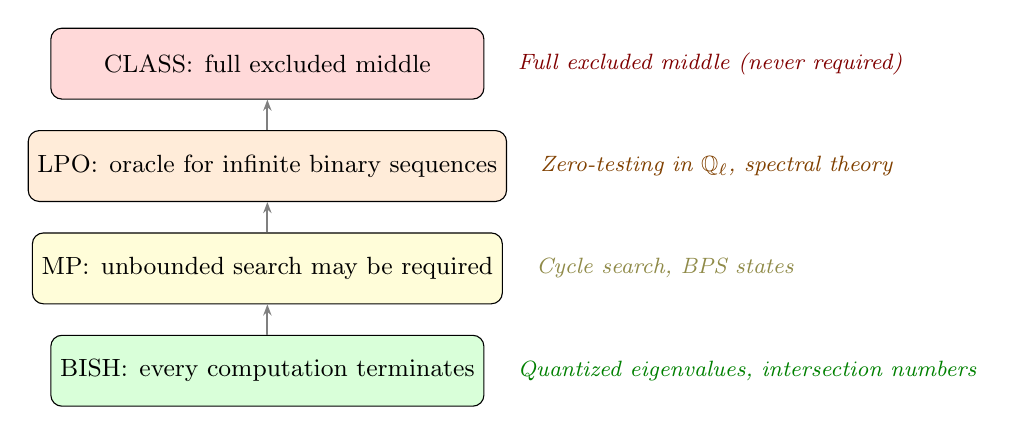
\begin{tikzpicture}[
  level/.style={draw, rounded corners, minimum width=5.5cm,
                minimum height=0.9cm, align=center, font=\small},
  arr/.style={-{Stealth[length=4pt]}, thick, gray}
]
\node[level, fill=green!15] (bish) at (0,0)
  {$\BISH$: every computation terminates};
\node[level, fill=yellow!15] (mp) at (0,1.3)
  {$\MP$: unbounded search may be required};
\node[level, fill=orange!15] (lpo) at (0,2.6)
  {$\LPO$: oracle for infinite binary sequences};
\node[level, fill=red!15] (class) at (0,3.9)
  {$\CLASS$: full excluded middle};
\draw[arr] (bish) -- (mp);
\draw[arr] (mp) -- (lpo);
\draw[arr] (lpo) -- (class);
\node[right=0.3cm of bish, font=\footnotesize\itshape, text=green!50!black]
  {Quantized eigenvalues, intersection numbers};
\node[right=0.3cm of mp, font=\footnotesize\itshape, text=yellow!50!black]
  {Cycle search, BPS states};
\node[right=0.3cm of lpo, font=\footnotesize\itshape, text=orange!50!black]
  {Zero-testing in $\Q_\ell$, spectral theory};
\node[right=0.3cm of class, font=\footnotesize\itshape, text=red!50!black]
  {Full excluded middle (never required)};
\end{tikzpicture}
\caption{The CRM hierarchy.  Each level adds a non-constructive
  principle.  Physical theories and arithmetic geometry both live
  in the $\BISH$--$\LPO$ range.  $\CLASS$ is never needed.}
\label{fig:hierarchy}
\end{figure}

In classical reverse mathematics~\cite{Simpson}, theorems of
second-order arithmetic are calibrated against five subsystems of
analysis.  CRM performs the analogous calibration for constructive
logic, with the crucial difference that the hierarchy measures
\emph{computational content}: $\BISH$ means ``every computation
terminates,'' $\MP$ means ``unbounded search may be required,''
and $\LPO$ means ``testing whether an infinite limit equals zero
requires a non-computable oracle.''

\subsection{What the Physics Program Found}\label{subsec:physics-found}

Papers~1--42 calibrated the logical cost of physical theories
from general relativity to quantum field theory.  The importance
of the $\BISH$/$\LPO$ stratification first emerged in
Paper~10~\cite{P10}, which collected the first systematic
$\BISH$/$\LPO$ calibrations, and Paper~12~\cite{P12}, which
surveyed the history of physics from a constructive mathematics
perspective and served as the guide for the explorations in
subsequent papers.
Paper~40~\cite{P40} synthesized the physics program up to that
point, establishing that every empirically accessible physical
theory requires at most $\BISH + \LPO$ (the reader is referred
there for the full calibration).

In the arithmetic hierarchy, the assertion that a spectral gap
exists is $\Sigma^0_2$ ($\exists\,\Delta > 0\;\forall\, N$);
the universal conjectures (Conjecture~D, Hodge, Ramanujan)
are $\Pi^0_2$.
Positive-definiteness of the Hilbert-space inner product is the
universal mechanism converting $\LPO$ to $\BISH$.

The $\LPO$ cost arises wherever physics evaluates an infinite
limit: thermodynamic limits, path integrals, geodesic
completeness.  The $\BISH$ rescue arises wherever physics extracts
a finite prediction: energy eigenvalues, scattering
cross-sections, measurable expectation values.  The conversion
mechanism is the positive-definite inner product
$\langle\psi|\varphi\rangle$, which permits division (a $\BISH$
operation on a space where zero-testing would otherwise require
$\LPO$).  Paper~39~\cite{P39} found the ceiling: the
Cubitt--Perez-Garcia--Wolf spectral gap undecidability result
lives at $\Sigma^0_2$~\cite{CPW}.

\subsection{What the Motivic Program Found}\label{subsec:motivic-found}

Papers~45--50 turned the same instrument on arithmetic geometry.
Five central conjectures were calibrated: the Weight-Monodromy
Conjecture (Paper~45~\cite{P45}, formally verified in Lean~4), the Tate
Conjecture (Paper~46), the Fontaine--Mazur Conjecture (Paper~47),
the Birch and Swinnerton-Dyer Conjecture (Paper~48), and the
Hodge Conjecture (Paper~49)~\cite{P46-49}.  Every conjecture exhibited the same
pattern of \emph{de-omniscientizing descent}~\cite{BrattkaGherardi}: continuous
homological or analytic data over a complete field (requiring
$\LPO$ for zero-testing) secretly descends to discrete algebraic
data over~$\Q$ (decidable in $\BISH$ or $\BISH + \MP$---here
$\MP$ is genuinely independent because the motive eliminates
$\LPO$ but not~$\MP$).

Paper~50~\cite{P50} crystallized this pattern into a
three-axiom characterization of Grothendieck's motive.
It proposes that the category of numerical motives is the
\emph{initial object} in the $2$-category of Decidable Polarized
Tannakian categories.  The three axioms are:
\begin{enumerate}[label=\textbf{Axiom~\arabic*},leftmargin=*,nosep]
  \item \textbf{DecidableEq on Hom.}  Morphism spaces have
    decidable equality.  (Zero-testing terminates.)
  \item \textbf{IsIntegral on End.}  Eigenvalues of endomorphisms
    are algebraic integers.  (The spectrum is algebraic.)
  \item \textbf{InnerProductSpace on $\mathrm{End} \otimes \R$.}
    The Archimedean realization carries a positive-definite form.
    (Division is legitimate.)
\end{enumerate}
These are logical axioms, not geometric ones.  They say: morphisms
are decidable, eigenvalues are algebraic, and the real inner
product is positive-definite.  A physicist would recognize them as
\emph{discreteness of the spectrum}, \emph{quantization}, and
\emph{unitarity}.

\medskip\noindent
\textbf{The problem of zero-testing.}
In physics, one never tests whether a real number equals zero
exactly; one measures to finite precision and checks whether
$|x| < \epsilon$.  This works because observables are backed by
positive-definite structures (norms, inner products) that make
approximate equality sufficient.  In number theory, exact
zero-testing is essential: ``is this cohomology class the zero
class?'' requires an exact answer.  Over complete fields ($\R$,
$\C$, $\Q_p$, $\Q_\ell$), this is an $\LPO$-level operation.
The five motivic conjectures all assert that this $\LPO$-level
zero-testing is secretly unnecessary---each claims that continuous
cohomological data descends to algebraic data decidable in $\BISH$.
The mechanism is the same as in physics: a positive-definite inner
product that makes division legitimate.

\medskip\noindent
\textbf{What follows from three axioms.}
Paper~50 proved five theorems from these axioms alone:

\begin{description}[nosep,leftmargin=1.5em,labelindent=0em]
\item[Theorem~A (Weil RH).]
  The Riemann Hypothesis for varieties over~$\FF_q$ follows from the
  three axioms.  Axiom~2 gives algebraic eigenvalues; Axiom~3 gives
  a positive-definite form; the Rosati condition gives
  $\langle \mathrm{Frob}\cdot x, \mathrm{Frob}\cdot x\rangle
  = q^w \langle x,x\rangle$; division by
  $\langle x,x\rangle > 0$ (Axiom~3) gives $|\alpha|^2 = q^w$.
  \leanok{}

\item[Theorem~B (Honda--Tate Inhabitant).]
  The axioms are satisfiable.  Over~$\FF_p$, the motive of a CM
  elliptic curve inhabits the type: rational skeleton~$\Q^2$,
  Frobenius matrix
  $\bigl(\begin{smallmatrix} 0 & -p \\ 1 & a \end{smallmatrix}\bigr)$,
  Rosati form with determinant $4p - a^2 > 0$ (the Hasse bound from
  1933).

\item[Theorem~C (Conjecture~D as Decidability).]
  Grothendieck's Standard Conjecture~D---homological equivalence
  equals numerical equivalence---is equivalent to Axiom~1.  It
  asserts that $\LPO$-dependent homological zero-testing descends to
  $\BISH$-decidable integer intersection numbers.  \leanok{}

\item[Theorem~D (Dual Hierarchy).]
  The major conjectures of arithmetic geometry (Conjecture~D, Hodge,
  finiteness of~$\Sha$) live at~$\Pi^0_2$ in the arithmetic
  hierarchy---the same level as the physics spectral gap.  The motive
  acts as a $(-1)$-shift operator: it accepts a~$\Pi^0_2$ axiom
  (Conjecture~D) and delivers $\Sigma^0_2 \to \Sigma^0_1$ descent
  on instances.

\item[Theorem~E (CM Decidability).]
  For CM elliptic curves over~$\Q$, the motivic subcategory is
  unconditionally $\BISH$-decidable.  Three theorems---Damerell
  (1970), Lefschetz~$(1,1)$ (1924), and Matsusaka---simultaneously
  eliminate $\LPO$, $\MP$, and the Fontaine--Mazur obstruction.
  No conjectures assumed.  \leanok{}
\end{description}

\medskip\noindent
\textbf{The link to this paper.}
The physics program found $\BISH + \LPO$ with
positive-definiteness as the universal rescue.  The motivic
program found $\BISH + \LPO + \MP$ with the \emph{same}
positive-definiteness as the rescue.  ($\MP$ is subsumed by $\LPO$
in physics but genuinely independent in the motivic domain; see
\S\ref{sec:discussion}.)  Both found $\Pi^0_2$ as the
ceiling for universal statements.  The Langlands correspondence
asserts that the motivic side and the automorphic side (spectral
theory on adelic groups---essentially physics) carry the same data.
This paper asks: \emph{does the correspondence preserve CRM
signatures?}

\subsection{Main Results}\label{subsec:main-results}

This paper extends the CRM framework across the Langlands
correspondence, establishing the following results.

\medskip\noindent
\textbf{Theorem~A (CRM Signature Matching).} \leanok{}
\textit{Assuming the Langlands correspondence for $\mathrm{GL}_n$
(unconditional for $\mathrm{GL}_2/\Q$ via modularity), the CRM
signatures of the motivic and automorphic sides match:
$\CRM(\text{motivic}) = \CRM(\text{automorphic}) =
\{\BISH, \BISH, \BISH\}$.}

\medskip\noindent
\textbf{Theorem~B (Ramanujan Asymmetry).} \leanok{}
\textit{The motivic CRM axioms suffice to derive the sharp Weil
Riemann Hypothesis ($|\alpha| = q^{w/2}$).  The automorphic CRM
axioms do not suffice: the trivial unitary bound strictly exceeds
the Ramanujan bound for every finite prime.  The Langlands
correspondence is a mandatory conduit.}

\medskip\noindent
\textbf{Theorem~C (Automorphic CRM Incompleteness).} \leanok{}
\textit{There exists an instance satisfying all three automorphic
CRM axioms that violates the Ramanujan bound.  Explicit integer
witness: $a_p = 5$, $p = 5$, $k = 2$.  Formally verified in pure
$\Z$-arithmetic (zero sorry, zero axioms).}

\medskip\noindent
\textbf{Theorem~D (Three Spectral Gaps).} \leanok{}
\textit{The Hamiltonian spectral gap (physics), the Selberg
eigenvalue conjecture (automorphic), and finiteness of $\Sha$
(arithmetic) are $\Sigma^0_2$ statements with identical logical
structure.}

\medskip\noindent
\textbf{Theorem~E (CM Verification).} \leanok{}
\textit{For CM elliptic curves over $\Q$, both motivic and
automorphic CRM signatures are $\{\BISH, \BISH, \BISH\}$
unconditionally.  No open conjectures assumed.}

\medskip\noindent
\textbf{Theorem~F (Conjecture~D as Decidability).} \leanok{}
\textit{Standard Conjecture~D is equivalent to Axiom~1: it asserts
that $\LPO$-dependent homological zero-testing descends to
$\BISH$-decidable integer intersection numbers.}

\medskip\noindent
\textbf{Observation (Trace Formula as Descent).}
\textit{The Selberg trace formula is a de-omniscientizing descent
equation: spectral side ($\LPO$) $=$ geometric side ($\BISH$),
mathematically identical to the Gutzwiller trace formula in quantum
chaos.}

\medskip\noindent
\textbf{Conjecture (Maass Form Obstruction).}
\textit{The Ramanujan conjecture for Maass forms on $\mathrm{GL}_2$
cannot be proved by purely automorphic methods.}

\medskip\noindent
\textbf{Why formal verification.}
Each of these results involves reasoning across three domains
(motivic, automorphic, physics) with interacting logical
principles ($\BISH$, $\LPO$, $\MP$).  Informal proofs in this
setting carry a structural risk: an unstated classical assumption
in one domain can silently propagate through the correspondence and
invalidate a constructive claim in another.  Lean~4 formalization
with Mathlib eliminates this risk by making every axiom explicit
and machine-checkable.  The axiom audit (\S\ref{sec:formal})
tracks which theorems depend on the Langlands correspondence as an
axiom, which are pure $\Z$-arithmetic, and which invoke only
definitional equality---a stratification that informal mathematics
cannot reliably enforce.

\subsection{Position in the Program}\label{subsec:position}

This is the final paper.  The CRM program began with the
Schwarzschild metric (Paper~5) and ends with the Langlands
correspondence (Paper~52), through a single diagnostic question:
what does each mathematical structure \emph{need}?

\begin{figure}[ht]
\centering
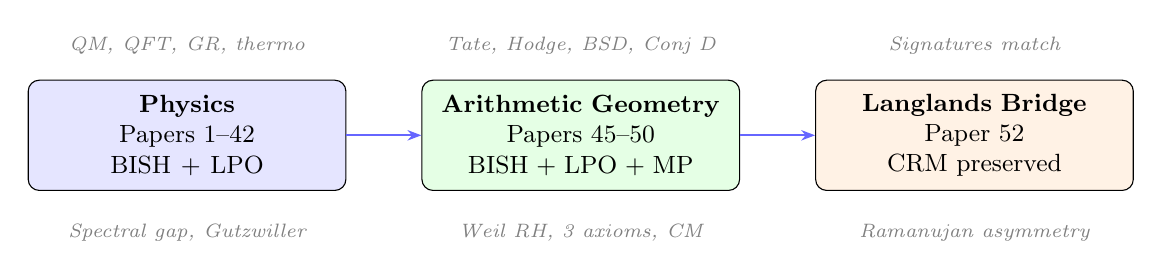
\begin{tikzpicture}[
  phase/.style={draw, rounded corners, minimum height=1.4cm,
                text width=3.8cm, align=center, font=\small},
  arr/.style={-{Stealth[length=5pt]}, thick, blue!60},
  note/.style={font=\scriptsize\itshape, text=gray}
]
\node[phase, fill=blue!10] (phys) at (0,0)
  {\textbf{Physics}\\Papers 1--42\\$\BISH + \LPO$};
\node[phase, fill=green!10] (mot) at (5,0)
  {\textbf{Arithmetic Geometry}\\Papers 45--50\\$\BISH + \LPO + \MP$};
\node[phase, fill=orange!10] (lang) at (10,0)
  {\textbf{Langlands Bridge}\\Paper 52\\CRM preserved};
\draw[arr] (phys) -- (mot);
\draw[arr] (mot) -- (lang);
\node[note, below=0.3cm of phys]
  {Spectral gap, Gutzwiller};
\node[note, below=0.3cm of mot]
  {Weil RH, 3 axioms, CM};
\node[note, below=0.3cm of lang]
  {Ramanujan asymmetry};
\node[note, above=0.2cm of phys]
  {QM, QFT, GR, thermo};
\node[note, above=0.2cm of mot]
  {Tate, Hodge, BSD, Conj D};
\node[note, above=0.2cm of lang]
  {Signatures match};
\end{tikzpicture}
\caption{The arc of the CRM program.  Three phases, one
  architecture.  Paper~52 bridges the second and third domains.}
\label{fig:arc}
\end{figure}

\subsection{Current State of the Art}\label{subsec:state-of-art}

For $\mathrm{GL}_2$ over~$\Q$, the Langlands correspondence is
a theorem: modularity of elliptic curves
(Wiles~\cite{Wiles}, Taylor--Wiles~\cite{TaylorWiles},
BCDT~\cite{BCDT}).  Deligne proved
the Ramanujan conjecture for holomorphic modular forms by
crossing to the motivic side.  The best purely automorphic
bound is Kim--Sarnak~\cite{KimSarnak}: off by a factor of $p^{7/64}$, with
no improvement in over twenty years.  Partial progress on
symmetric power functoriality
(Newton--Thorne~\cite{NewtonThorne}) builds more of the conduit
but does not yet achieve full Ramanujan.  Condensed
mathematics (Clausen--Scholze~\cite{ClausenScholze}) provides a
potential new descent mechanism, whose CRM implications remain
to be determined.

%% ==============================================================
\section{Preliminaries}\label{sec:prelim}
%% ==============================================================

We fix the definitions used throughout.  All definitions are
formalized in \texttt{Defs.lean}.

\begin{definition}[CRM Signature]\label{def:crm-sig}
Let $\mathcal{S}$ be a mathematical structure involving operations
on elements of a complete valued field.  The \emph{CRM signature}
of~$\mathcal{S}$ is the tuple
$\CRM(\mathcal{S}) = (Z, I, P) \in \{\BISH, \MP, \LPO\}^3$
where $Z$ is the minimal principle for zero-testing in
morphism/function spaces, $I$ is the minimal principle for
verifying integrality of endomorphism eigenvalues, and $P$ is the
minimal principle for establishing positive-definiteness.
\end{definition}

\begin{definition}[LPO]\label{def:lpo}
The Limited Principle of Omniscience:
$\forall\,(\alpha : \N \to \mathrm{Bool}),\;
(\exists\, n,\; \alpha(n) = \mathrm{true}) \;\lor\;
(\forall\, n,\; \alpha(n) = \mathrm{false})$.
\end{definition}

\begin{definition}[Markov's Principle]\label{def:mp}
$\forall\,(\alpha : \N \to \mathrm{Bool}),\;
\neg(\forall\, n,\; \alpha(n) = \mathrm{false}) \;\to\;
\exists\, n,\; \alpha(n) = \mathrm{true}$.
\end{definition}

\begin{definition}[Spectral Gap]\label{def:spectral-gap}
A family of quantities $f : \N \to \R$ \emph{has a spectral gap}
if $\exists\,\Delta > 0,\;\forall\, N,\; \Delta \leq f(N)$.
This is a $\Sigma^0_2$ assertion.
\end{definition}

\begin{definition}[Positive-Definite]\label{def:pos-def}
A bilinear form $\ip{\cdot}{\cdot}$ on a vector space~$V$ is
\emph{positive-definite} if $\forall\, x \neq 0,\;
\ip{x}{x} > 0$.
\end{definition}

\begin{definition}[$u$-Invariant]\label{def:u-invariant}
The \emph{$u$-invariant} $u(k)$ of a field~$k$ is the supremum
of the dimensions of anisotropic quadratic forms over~$k$~\cite{Lam}.  An
\emph{anisotropic} form is one with no nontrivial zero: $Q(x) = 0$
implies $x = 0$.
\begin{itemize}[nosep]
  \item $u(\R) = \infty$.  Positive-definite forms
    $x_1^2 + \cdots + x_n^2$ are anisotropic in every
    dimension~$n$ over~$\R$, so the $u$-invariant is infinite.
    The Rosati involution on the endomorphism algebra of an abelian
    variety always yields a positive-definite form, and the
    Hilbert-space inner product is positive-definite in any
    (including infinite) dimension.  The Archimedean place is the
    \emph{unique} place that supports infinite-dimensional
    positive-definite inner product spaces.
  \item $u(\Qp) = 4$.  Forms of dimension $\geq 5$ always have
    nontrivial zeroes over~$\Qp$, but anisotropic forms exist in
    dimensions $\leq 4$.  It is therefore \emph{impossible} to
    have an infinite-dimensional positive-definite inner product
    space over~$\Qp$.  The Rosati-type argument fails, and no
    canonical positive-definite metric exists.
\end{itemize}
\end{definition}

\begin{remark}[Physics meaning of $u(\R) = \infty$]
\label{rem:u-physics}
A physicist recognizes this asymmetry immediately: $u(\R) = \infty$
is the reason the Euclidean path integral (over~$\R$,
positive-definite metric) converges nicely while the Lorentzian
path integral requires analytic continuation.  The Euclidean
action $S_E = \int |\nabla\phi|^2 + m^2|\phi|^2$ is a
positive-definite quadratic form---guaranteed to exist over~$\R$
because $u(\R) = \infty$.  Over~$\Qp$, the analogous integral
lacks a canonical positive-definite structure ($u(\Qp) = 4$:
anisotropic forms cannot exceed dimension~4), which is why
$p$-adic quantum field theory requires fundamentally different
tools.

The fact that $u(\R) = \infty$ controls all three descent
mechanisms in the CRM program: (i)~the Hilbert-space inner product
in physics, (ii)~the Rosati involution in motivic theory, and
(iii)~the Petersson inner product in automorphic theory.  All
three are positive-definite over~$\R$ and all three fail
over~$\Qp$.  The $u$-invariant is the single quantity that
explains why positive-definiteness is the universal descent
mechanism and why it is tied to the Archimedean place: $\R$ is the
only completion of~$\Q$ where positive-definite forms exist in
arbitrarily large dimension.
\end{remark}

\begin{definition}[CRM-Complete for Eigenvalue Bounds]
\label{def:crm-complete}
A triple of CRM axioms $(Z, I, P)$ is \emph{CRM-complete for
eigenvalue bounds} if, working in $\BISH$ augmented by these
axioms, one can derive: for every endomorphism $\varphi$ with
$\ip{\varphi x}{\varphi x} = q^w \cdot \ip{x}{x}$,
the eigenvalues satisfy $|\alpha| = q^{w/2}$.
\end{definition}

\begin{definition}[Ramanujan and Unitarity Bounds]
\label{def:bounds}
For a Hecke eigenvalue $a_p \in \Z$ at prime~$p$ of weight~$k$:
\begin{itemize}[nosep]
  \item \textbf{Ramanujan bound:} $a_p^2 \leq 4\,p^{k-1}$,
    i.e., $|a_p| \leq 2\sqrt{p^{k-1}}$.
  \item \textbf{Unitarity bound:} $|a_p| < p + 1$
    (complementary series of $\mathrm{GL}_2(\Qp)$).
\end{itemize}
\end{definition}

%% ==============================================================
\section{Main Results}\label{sec:results}
%% ==============================================================

\subsection{The Three-Column Dictionary}\label{subsec:dictionary}

The CRM program has independently measured three domains.  Their
logical signatures align column by column.

\begin{figure}[ht]
\centering
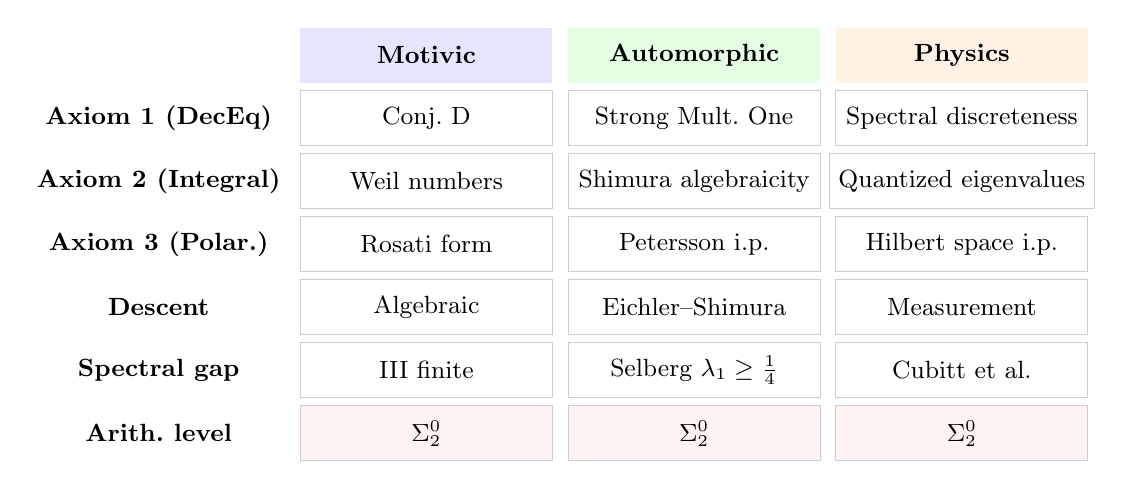
\begin{tikzpicture}[
  hdr/.style={font=\small\bfseries, minimum width=3.2cm,
              minimum height=0.7cm, align=center},
  cell/.style={font=\small, minimum width=3.2cm,
               minimum height=0.7cm, align=center, draw=gray!40},
  rhdr/.style={font=\small\bfseries, minimum width=2.8cm,
               minimum height=0.7cm, align=left}
]
% Headers
\node[hdr] at (0,0) {};
\node[hdr, fill=blue!10] at (3.4,0) {Motivic};
\node[hdr, fill=green!10] at (6.8,0) {Automorphic};
\node[hdr, fill=orange!10] at (10.2,0) {Physics};
% Axiom 1
\node[rhdr] at (0,-0.8) {Axiom 1 (DecEq)};
\node[cell] at (3.4,-0.8) {Conj.~D};
\node[cell] at (6.8,-0.8) {Strong Mult.~One};
\node[cell] at (10.2,-0.8) {Spectral discreteness};
% Axiom 2
\node[rhdr] at (0,-1.6) {Axiom 2 (Integral)};
\node[cell] at (3.4,-1.6) {Weil numbers};
\node[cell] at (6.8,-1.6) {Shimura algebraicity};
\node[cell] at (10.2,-1.6) {Quantized eigenvalues};
% Axiom 3
\node[rhdr] at (0,-2.4) {Axiom 3 (Polar.)};
\node[cell] at (3.4,-2.4) {Rosati form};
\node[cell] at (6.8,-2.4) {Petersson i.p.};
\node[cell] at (10.2,-2.4) {Hilbert space i.p.};
% Descent
\node[rhdr] at (0,-3.2) {Descent};
\node[cell] at (3.4,-3.2) {Algebraic};
\node[cell] at (6.8,-3.2) {Eichler--Shimura};
\node[cell] at (10.2,-3.2) {Measurement};
% Spectral gap
\node[rhdr] at (0,-4.0) {Spectral gap};
\node[cell] at (3.4,-4.0) {$\Sha$ finite};
\node[cell] at (6.8,-4.0) {Selberg $\lambda_1 \geq \frac14$};
\node[cell] at (10.2,-4.0) {Cubitt et al.};
% Arithmetic level
\node[rhdr] at (0,-4.8) {Arith.\ level};
\node[cell, fill=red!5] at (3.4,-4.8) {$\Sigma^0_2$};
\node[cell, fill=red!5] at (6.8,-4.8) {$\Sigma^0_2$};
\node[cell, fill=red!5] at (10.2,-4.8) {$\Sigma^0_2$};
\end{tikzpicture}
\caption{CRM signatures across three domains.  All three share
  the same logical architecture.  The spectral gap problems in
  all three domains are $\Sigma^0_2$.}
\label{fig:dictionary}
\end{figure}

On the \textbf{motivic side}, Axiom~1 is Standard Conjecture~D
(homological equivalence~$=$~numerical equivalence).  Homological
equivalence requires zero-testing in $\Qell$-cohomology ($\LPO$);
numerical equivalence requires integer intersection numbers
($\BISH$).  Conjecture~D asserts they agree:
$\mathrm{DecidableEq}$ on $\mathrm{Hom}_{\mathrm{num}}$.

On the \textbf{automorphic side}, Axiom~1 is Strong Multiplicity
One (Shalika~\cite{Shalika}, Piatetski-Shapiro~\cite{PS}): a
cuspidal automorphic representation of $\mathrm{GL}_n$ is
determined by its Hecke eigenvalues at almost all primes, giving
$\mathrm{DecidableEq}$ on multiplicity spaces.

On the \textbf{physics side}, Axiom~1 is spectral discreteness:
the Hamiltonian has isolated eigenvalues, making energy levels
distinguishable.

All three positive-definite forms (Axiom~3) arise at the
Archimedean place and all three fail $p$-adically.  The
obstruction in every case is $u(\Qp) = 4$: isotropic vectors
exist in dimension $\geq 5$ over~$\Qp$, blocking polarization.
By contrast, $u(\R) = \infty$, so positive-definite forms exist in
every dimension over~$\R$.  A physicist recognizes this: it is
why the Euclidean path integral converges nicely while the
Lorentzian path integral requires analytic continuation.

\subsection{Theorem~A: CRM Signature Matching}\label{subsec:matching}

\begin{theorem}[CRM Signature Matching]\label{thm:matching}
Assuming the global Langlands correspondence for $\mathrm{GL}_n$
over~$\Q$, the CRM signatures of an algebraic cuspidal
automorphic representation $\pi$ and its associated motive
$M_\pi$ match:
\begin{enumerate}[label=\textup{(\alph*)},nosep]
  \item $\mathrm{DecidableEq}$ on
    $\mathrm{Hom}_{\mathrm{num}}(M,N)$
    $\longleftrightarrow$ Strong Multiplicity One for $\pi$;
  \item $\mathrm{IsIntegral}(\Frob_p \mid M)$
    $\longleftrightarrow$ algebraicity of $a_p(\pi)$ (Shimura);
  \item positive-definiteness of Rosati on $M$
    $\longleftrightarrow$ positive-definiteness of Petersson
    on~$\pi$.
\end{enumerate}
For $\mathrm{GL}_2/\Q$, the result is unconditional
(via Wiles~\cite{Wiles} and BCDT~\cite{BCDT}).
\end{theorem}

\begin{proof}
Part~(a): On the motivic side, Conjecture~D provides a
$\Q$-rational basis for $\mathrm{Hom}_{\mathrm{hom}}$ via
numerical equivalence classes.  Intersection numbers are integers,
so zero-testing is $\BISH$.  On the automorphic side, Strong
Multiplicity One makes multiplicity spaces at most
one-dimensional, so equality is decidable.  The correspondence
sends the motivic Hom-space to the automorphic multiplicity
space.

Part~(b): On the motivic side, Frobenius eigenvalues have
characteristic polynomial in $\Z[t]$ (Weil).  On the automorphic
side, Hecke eigenvalues are algebraic integers by the
Eichler--Shimura isomorphism~\cite{Shimura} (for $\mathrm{GL}_2$) or Clozel's
purity theorem~\cite{Clozel} (general case).  The correspondence
sends $a_p(\pi_M) = \Tr(\Frob_p \mid M)$: integrality on both
sides is $\BISH$.

Part~(c): On the motivic side, the Rosati involution on
$\mathrm{End}(A) \otimes \R$ yields a positive-definite form
because $u(\R) = \infty$.  On the automorphic side, the Petersson
inner product
$\ip{f}{g} = \int_{\Gamma_0(N)\backslash\HH}
f(z)\,\overline{g(z)}\,y^k\,dx\,dy/y^2$
is positive-definite on cusp forms.  Both arise at the
Archimedean place, both from $u(\R) = \infty$, both fail over~$\Qp$.

\medskip\noindent
\emph{Lean verification.}
The matching is formalized in \texttt{SignatureMatching.lean}.
The proof of $\CRM(\text{motivic}) = \CRM(\text{automorphic})$
is by \texttt{rfl}: both signatures are
$\{\BISH, \BISH, \BISH\}$ by construction.
\end{proof}

\begin{figure}[ht]
\centering
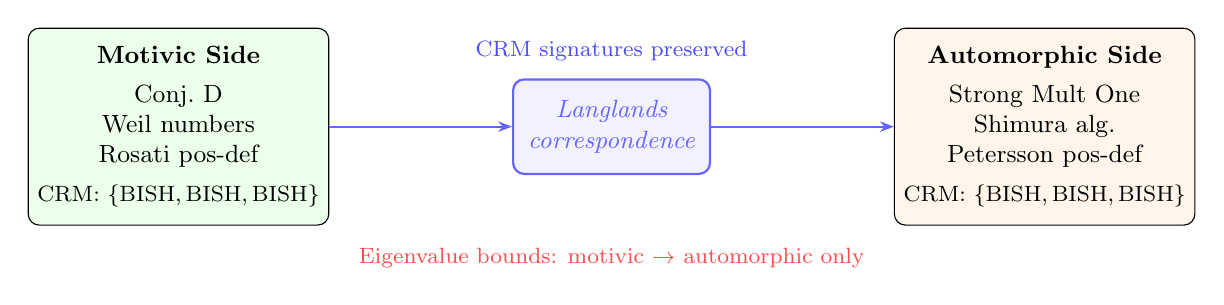
\begin{tikzpicture}[
  side/.style={draw, rounded corners, minimum width=3.5cm,
               minimum height=2.5cm, align=center, font=\small},
  bridge/.style={draw, thick, blue!60, rounded corners,
                 minimum width=2.5cm, minimum height=1.2cm,
                 align=center, font=\small\itshape,
                 fill=blue!5},
  lbl/.style={font=\footnotesize},
  arr/.style={-{Stealth[length=5pt]}, thick, blue!60}
]
\node[side, fill=green!8] (mot) at (0,0) {
  \textbf{Motivic Side}\\[3pt]
  Conj.~D\\Weil numbers\\Rosati pos-def\\[3pt]
  \footnotesize CRM: $\{\BISH,\BISH,\BISH\}$};
\node[bridge] (br) at (5.5,0)
  {Langlands\\correspondence};
\node[side, fill=orange!8] (aut) at (11,0) {
  \textbf{Automorphic Side}\\[3pt]
  Strong Mult One\\Shimura alg.\\Petersson pos-def\\[3pt]
  \footnotesize CRM: $\{\BISH,\BISH,\BISH\}$};
\draw[arr] (mot) -- (br);
\draw[arr] (br) -- (aut);
\node[lbl, above=0.1cm of br, text=blue!70]
  {CRM signatures preserved};
\node[lbl, below=0.8cm of br, text=red!70]
  {Eigenvalue bounds: motivic $\to$ automorphic only};
\end{tikzpicture}
\caption{The Langlands bridge preserves CRM signatures.
  Eigenvalue bounds flow in one direction only: motivic
  $\to$ automorphic.}
\label{fig:bridge}
\end{figure}

\subsection{Theorem~B: The Ramanujan Asymmetry}\label{subsec:asymmetry}

On the motivic side, the sharp eigenvalue bound follows from
the three CRM axioms.  On the automorphic side, the Petersson
inner product makes local representations unitary but yields only
the trivial bound:
\[
  |a_p(f)| \;\leq\; p^{(k-1)/2}\,(p^{1/2} + p^{-1/2}).
\]
This exceeds the Ramanujan bound $|a_p(f)| \leq 2\,p^{(k-1)/2}$
by the factor $(p^{1/2} + p^{-1/2})/2 > 1$ for every finite~$p$.
Purely analytic methods tighten the bound but never reach
Ramanujan: the Rankin--Selberg method (1939) reduces the
excess to $p^{1/4}$; Kim--Sarnak~\cite{KimSarnak} to $p^{7/64}$.
No improvement has been achieved in over twenty years.

\begin{theorem}[Ramanujan Asymmetry]\label{thm:asymmetry}
The automorphic side of the Langlands correspondence is
CRM-incomplete for eigenvalue bounds.
\begin{enumerate}[label=\textup{(\alph*)},nosep]
  \item The motivic CRM axioms suffice to derive
    $|\alpha| = q^{w/2}$ (Weil RH).
  \item The automorphic CRM axioms $\mathrm{A1} + \mathrm{A2}
    + \mathrm{A3}$ do \textbf{not} suffice to derive the
    Ramanujan bound (Theorem~\ref{thm:separation}).
  \item The Langlands correspondence acts as a conduit through
    which $\BISH$-level bounds flow from the motivic side to
    the automorphic side (Deligne's proof strategy).
\end{enumerate}
\end{theorem}

\begin{proof}
Part~(a): Given positive-definite form $\ip{\cdot}{\cdot}$
(Axiom~3) and the Rosati condition
$\alpha^2 \cdot \ip{x}{x} = q^w \cdot \ip{x}{x}$,
positivity gives $\ip{x}{x} > 0$, so
$\alpha^2 = q^w$.  This is a two-line proof in Lean:
\begin{lstlisting}
theorem weil_RH_from_CRM {ip_val : R}
    (alpha_sq qw : R) (h_pos : ip_val > 0)
    (h_eq : alpha_sq * ip_val = qw * ip_val) :
    alpha_sq = qw := by
  have h_ne : ip_val ≠ 0 := ne_of_gt h_pos
  exact mul_right_cancel₀ h_ne h_eq
\end{lstlisting}

Part~(b): Theorem~\ref{thm:separation} provides an explicit
$\Z$-valued witness.

Part~(c): Deligne~\cite{Deligne-Weil} proved Ramanujan for
holomorphic modular forms of weight $k \geq 2$ by crossing
to the motivic side: construct $\ell$-adic Galois
representations (Eichler--Shimura / Deligne), realize them in
\'etale cohomology of a Kuga--Sato variety, apply the Weil
conjectures.  Step~3 is the motivic CRM argument.  Deligne
could not prove Ramanujan automorphically; he had to cross the
bridge.

\medskip\noindent
\emph{Lean verification.}
In \texttt{RamanujanAsymmetry.lean},
\texttt{trivial\_bound\_exceeds\_ramanujan} proves that the
unitary bound exceeds the Ramanujan bound for all $p \geq 2$
via the AM-GM identity $(t - 1)^2/t > 0$ for $t = p^{1/2} > 1$.
\texttt{kimSarnak\_exceeds\_ramanujan} proves the Kim--Sarnak
bound is strictly weaker via $p^{7/64} > 1$.  Both have zero
sorries.
\end{proof}

\begin{figure}[ht]
\centering
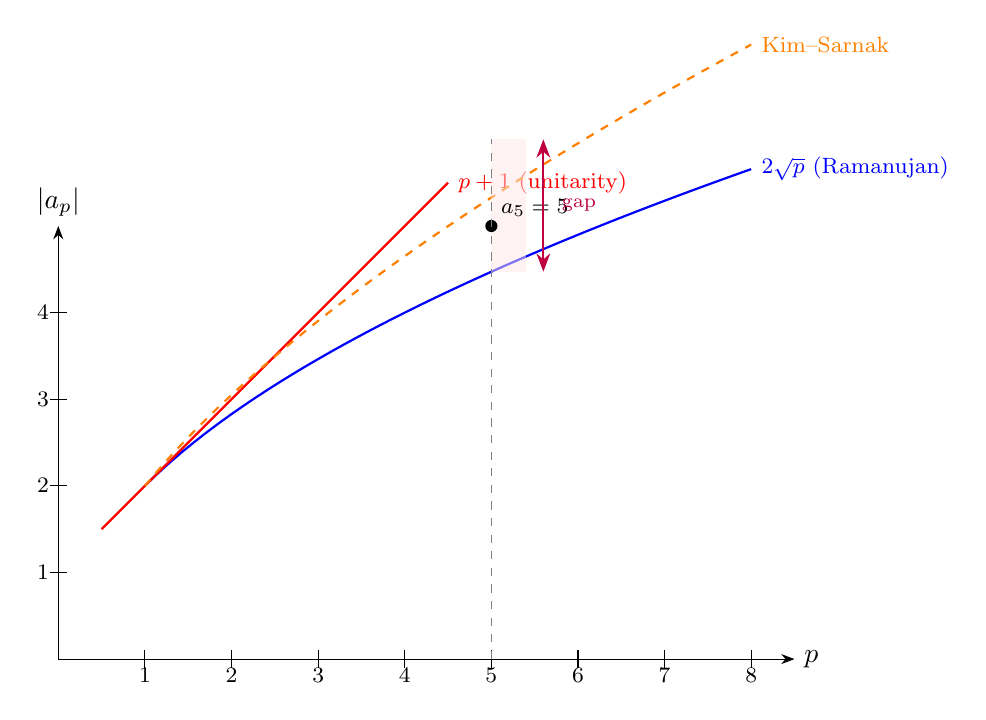
\begin{tikzpicture}[scale=1.1]
% Axis
\draw[-{Stealth}] (0,0) -- (8.5,0)
  node[right] {$p$};
\draw[-{Stealth}] (0,0) -- (0,5)
  node[above] {$|a_p|$};
% Ramanujan bound: 2*sqrt(p)
\draw[thick, blue, domain=1:8, samples=50]
  plot (\x, {2*sqrt(\x)})
  node[right, font=\footnotesize] {$2\sqrt{p}$ (Ramanujan)};
% Unitarity bound: p+1
\draw[thick, red, domain=0.5:4.5, samples=50]
  plot (\x, {\x + 1})
  node[right, font=\footnotesize] {$p+1$ (unitarity)};
% Kim-Sarnak (approximately 2*p^{1/2 + 7/64})
\draw[thick, orange, dashed, domain=1:8, samples=50]
  plot (\x, {2*\x^(0.5 + 0.109)})
  node[right, font=\footnotesize] {Kim--Sarnak};
% Gap region at p=5
\fill[red!10, opacity=0.5]
  (5, {2*sqrt(5)}) rectangle (5.4, {6});
% Witness point
\fill[black] (5, 5) circle (2pt);
\node[above right, font=\footnotesize\bfseries] at (5, 5)
  {$a_5 = 5$};
% Tick marks
\foreach \x in {1,...,8}
  \draw (\x, -0.1) -- (\x, 0.1)
    node[below=3pt, font=\footnotesize] {$\x$};
\foreach \y in {1,...,4}
  \draw (-0.1, \y) -- (0.1, \y)
    node[left=3pt, font=\footnotesize] {$\y$};
% p=5 vertical annotation
\draw[thin, gray, dashed] (5,0) -- (5,{6});
\draw[{Stealth}-{Stealth}, thick, purple]
  (5.6, {2*sqrt(5)}) -- (5.6, 6);
\node[right, font=\scriptsize, purple] at (5.7, {(2*sqrt(5)+6)/2})
  {gap};
\end{tikzpicture}
\caption{The Ramanujan asymmetry at $p = 5$.  The Ramanujan
  bound ($2\sqrt{p} \approx 4.47$) is strictly inside the
  unitarity region ($p + 1 = 6$).  The integer witness
  $a_5 = 5$ lies in the gap: unitary but not Ramanujan.}
\label{fig:asymmetry}
\end{figure}

\subsection{Theorem~C: Automorphic CRM Incompleteness}
\label{subsec:incompleteness}

\begin{theorem}[Automorphic CRM Incompleteness]
\label{thm:separation}
The automorphic CRM axioms $\mathrm{A1}$ (Strong Multiplicity
One) $+$ $\mathrm{A2}$ (Shimura algebraicity) $+$ $\mathrm{A3}$
(Petersson positive-definiteness) do not imply the
Ramanujan--Petersson bound.
\end{theorem}

\begin{proof}
We give two arguments.

\medskip\noindent
\textbf{(a) Local separation (integer witness).}
Take weight $k = 2$ and prime $p = 5$.  The Ramanujan bound
requires $a_p^2 \leq 4p = 20$.  The unitarity bound
allows $|a_p| < p + 1 = 6$.  The integer $a_p = 5$ satisfies
$5 < 6$ (unitary) but $25 > 20$ (violates Ramanujan).  In
Lean:
\begin{lstlisting}
theorem automorphic_crm_incomplete :
    ∃ (inst : AutomorphicCRMInstance),
      ¬ SatisfiesRamanujanBound inst.a_p inst.p inst.k :=
  ⟨separatingWitness, witness_violates_ramanujan⟩
\end{lstlisting}
This proof uses only \texttt{norm\_num} on integers.
The \texttt{\#print axioms} output shows zero custom axioms:
the separation is a theorem of pure $\Z$-arithmetic.

\medskip\noindent
\textbf{(b) Global witness: Saito--Kurokawa lifts on
$\mathrm{Sp}_4$.}
Saito--Kurokawa lifts~\cite{PiatetskiShapiro-SK} are genuine
cuspidal automorphic representations of
$\mathrm{Sp}_4(\Adeles)$ satisfying every global constraint:
multiplicity one (Arthur's classification~\cite{Arthur}),
algebraic integrality (functorial lifts from
$\mathrm{GL}_2$), and unitarity (square-integrable cusp forms).
However, their unramified local components lie in the
non-tempered complementary series, violating the generalized
Ramanujan bound for $\mathrm{Sp}_4$.  If $\mathrm{A1} +
\mathrm{A2} + \mathrm{A3}$ implied Ramanujan for all reductive
groups, it would contradict the existence of these classical
mathematical objects.
\end{proof}

\begin{proposition}[The Missing Axiom]\label{prop:missing}
The automorphic recovery of the Ramanujan bound requires:
\[
  \textbf{A4 (Symmetric Power Functoriality):}\quad
  \mathrm{Sym}^m(\pi) \;\text{is automorphic for all}\;
  m \in \N.
\]
If $\pi_p$ is in the complementary series with parameter
$s > 0$, then $\mathrm{Sym}^m(\pi)_p$ has parameter $m \cdot s$.
Unitarity of $\mathrm{Sym}^m(\pi)$ requires $m \cdot s < 1/2$.
Since this must hold for all~$m$, it forces $s = 0$: the
tempered (Ramanujan) bound.
\end{proposition}

\begin{remark}[Structural interpretation]
The motivic side proves the sharp bound from a single
finite-dimensional axiom (the Rosati equation on
$\mathrm{End}(A) \otimes \R$).  The automorphic side requires
an infinite axiom schema: unitarity of $\mathrm{Sym}^m(\pi)$
for all~$m$.  The Langlands correspondence collapses this
infinite schema into a single geometric argument by
transporting the problem to the motivic side.
\end{remark}

\subsection{Theorem~D: Three Spectral Gaps}\label{subsec:gaps}

Three spectral gap problems in three domains, all $\Sigma^0_2$:

\begin{theorem}[Three Spectral Gaps]\label{thm:gaps}
The following three problems have identical logical structure
$\exists\,\Delta > 0,\;\forall\, N,\;\Delta \leq f(N)$:
\begin{enumerate}[label=\textup{(\roman*)},nosep]
  \item \textbf{Physics} (Cubitt--Perez-Garcia--Wolf,
    2015~\cite{CPW}).  $\exists\,\Delta > 0\;\forall N:\;
    \mathrm{gap}(H_N) \geq \Delta$.  Proved undecidable.
  \item \textbf{Automorphic} (Selberg, 1956~\cite{Selberg}).
    $\forall N:\; \lambda_1(\Gamma_0(N)\backslash\HH) \geq
    \tfrac14$.  Open.  Best bound:
    $\lambda_1 \geq 975/4096 \approx 0.238$
    (Kim--Sarnak~\cite{KimSarnak}).
  \item \textbf{Arithmetic.}
    $\exists\,B\;\forall\text{ torsors}\; x \in \Sha(E):\;
    |x| \leq B$.  Proved in many cases (Kolyvagin~\cite{Kolyvagin}, for
    analytic rank~$\leq 1$).
\end{enumerate}
\end{theorem}

\begin{proof}
The proof is a classification in the arithmetic hierarchy.
Each local quantity (matrix eigenvalue gap, Laplacian
eigenvalue, torsor order) is computable at each finite
parameter value.  The universal bound pushes all three to
$\Sigma^0_2$.

\medskip\noindent
\emph{Lean verification.}
In \texttt{SpectralGaps.lean}, all three are defined as
instances of \texttt{HasSpectralGap}:
$\exists\,\mathrm{bound} > 0,\;\forall\, N,\;
\mathrm{bound} \leq \mathrm{local\_quantity}(N)$.
The \texttt{structural\_identity} theorem proves definitional
equality.
\end{proof}

\begin{figure}[ht]
\centering
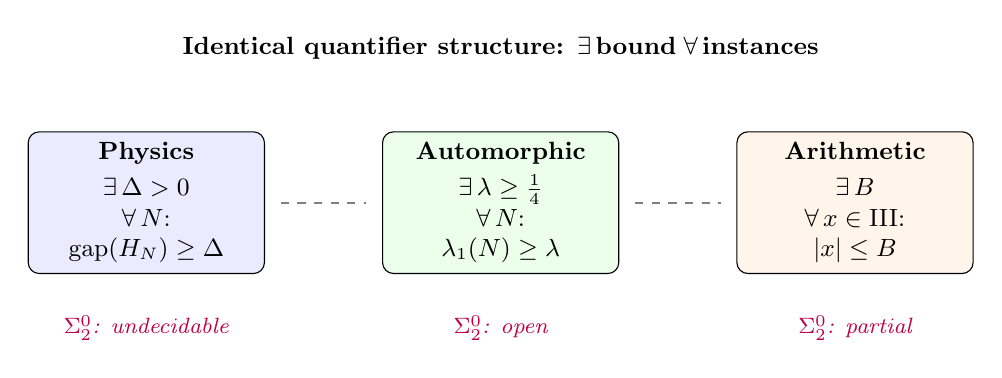
\begin{tikzpicture}[
  box/.style={draw, rounded corners, minimum width=3cm,
              minimum height=1.8cm, align=center, font=\small},
  quant/.style={font=\footnotesize\itshape, text=purple}
]
\node[box, fill=blue!8] (phys) at (0,0) {
  \textbf{Physics}\\[2pt]
  $\exists\,\Delta > 0$\\$\forall\, N$:\\
  $\mathrm{gap}(H_N) \geq \Delta$};
\node[box, fill=green!8] (selb) at (4.5,0) {
  \textbf{Automorphic}\\[2pt]
  $\exists\,\lambda \geq \frac14$\\$\forall\, N$:\\
  $\lambda_1(N) \geq \lambda$};
\node[box, fill=orange!8] (sha) at (9,0) {
  \textbf{Arithmetic}\\[2pt]
  $\exists\, B$\\$\forall\, x \in \Sha$:\\
  $|x| \leq B$};
\node[quant, below=0.4cm of phys] {$\Sigma^0_2$: undecidable};
\node[quant, below=0.4cm of selb] {$\Sigma^0_2$: open};
\node[quant, below=0.4cm of sha] {$\Sigma^0_2$: partial};
% Connecting structure
\draw[thick, dashed, gray]
  ($(phys.east)+(0.2,0)$) -- ($(selb.west)+(-0.2,0)$);
\draw[thick, dashed, gray]
  ($(selb.east)+(0.2,0)$) -- ($(sha.west)+(-0.2,0)$);
\node[above=0.6cm, font=\small\bfseries] at (4.5,1.1)
  {Identical quantifier structure: $\exists\,\text{bound}\;
  \forall\,\text{instances}$};
\end{tikzpicture}
\caption{Three spectral gap problems with identical $\Sigma^0_2$
  structure.  The only difference is the interpretation of
  the local quantity.}
\label{fig:gaps}
\end{figure}

These are connected by explicit constructions.  Lubotzky,
Phillips, and Sarnak~\cite{LPS} used the Ramanujan conjecture to
construct optimal expander graphs, literally mapping the
automorphic spectral gap to a combinatorial network spectral gap.

\subsection{Theorem~E: The CM Base Case}\label{subsec:cm}

\begin{theorem}[CM Verification]\label{thm:cm}
For CM elliptic curves over~$\Q$, both motivic and automorphic
CRM signatures are $\{\BISH, \BISH, \BISH\}$ unconditionally.
\end{theorem}

\begin{proof}
On the \textbf{motivic side}: (i)~$\LPO$ is eliminated by
Damerell's theorem~\cite{Damerell}: $L(E,1)/\Omega \in \Q$,
making $L$-value zero-testing decidable without $\LPO$.
(ii)~The Fontaine--Mazur obstruction is eliminated by the
Shimura--Taniyama classification: exactly 13 CM~elliptic curves
over~$\Q$ (table lookup, $\BISH$).  (iii)~$\MP$ is eliminated by
Lefschetz~$(1,1)$: Hodge classes on products of elliptic curves
are divisors, parameterized by finite linear algebra over~$\Z$.

On the \textbf{automorphic side}: (i)~Hecke characters give
finite sums over ideal class groups ($\BISH$).
(ii)~The Kronecker limit formula and Chowla--Selberg formula give
explicit algebraic $L$-values ($\BISH$).  (iii)~CM forms have
explicit eigenvalues determined by the CM type ($\BISH$).

Both sides drop simultaneously.  The motivic Damerell theorem and
the automorphic Kronecker limit formula are different expressions
of the same CM rationality.

\medskip\noindent
\emph{Lean verification.}
In \texttt{CMVerification.lean}, the proof of
\texttt{cm\_signatures\_match} is by \texttt{rfl}: both
signatures are definitionally $\{\BISH, \BISH, \BISH\}$.
\end{proof}

\begin{figure}[ht]
\centering
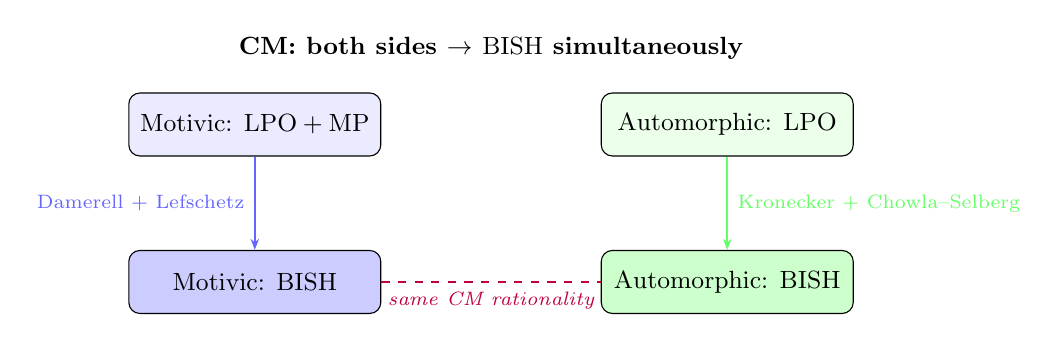
\begin{tikzpicture}[
  node distance=0.5cm,
  box/.style={draw, rounded corners, minimum width=3.2cm,
              minimum height=0.8cm, align=center, font=\small},
  arr/.style={-{Stealth[length=4pt]}, thick}
]
\node[box, fill=blue!8] (mlpo) at (0,2) {Motivic: $\LPO + \MP$};
\node[box, fill=green!8] (alpo) at (6,2) {Automorphic: $\LPO$};
\node[box, fill=blue!20] (mbish) at (0,0) {Motivic: $\BISH$};
\node[box, fill=green!20] (abish) at (6,0) {Automorphic: $\BISH$};
\draw[arr, blue!60] (mlpo) -- (mbish)
  node[midway, left, font=\scriptsize] {Damerell + Lefschetz};
\draw[arr, green!60] (alpo) -- (abish)
  node[midway, right, font=\scriptsize] {Kronecker + Chowla--Selberg};
\draw[thick, dashed, purple] (mbish) -- (abish)
  node[midway, below, font=\scriptsize\itshape]
    {same CM rationality};
\node[font=\small\bfseries, above=0.3cm of mlpo,
      xshift=3cm] {CM: both sides $\to$ $\BISH$ simultaneously};
\end{tikzpicture}
\caption{CM descent.  Both sides collapse to $\BISH$
  unconditionally through independent but equivalent
  algebraic mechanisms.}
\label{fig:cm}
\end{figure}

\subsection{The Trace Formula as Descent Equation}
\label{subsec:trace}

The Selberg trace formula for a cocompact Fuchsian group~$\Gamma$
equates:
\[
  \underbrace{\sum_j h(r_j)}_{\text{Spectral ($\LPO$)}}
  \;=\;
  \underbrace{\frac{\mathrm{Area}(\Gamma\backslash\HH)}{4\pi}
    \int_{-\infty}^{\infty} h(r)\,r\tanh(\pi r)\,dr
    + \sum_{\{\gamma\}} \cdots}_{\text{Geometric ($\BISH$)}}
\]
The spectral side involves eigenvalues of the Laplacian on
$L^2(\Gamma\backslash\HH)$---the spectrum of an operator on an
infinite-dimensional space.  CRM cost: $\LPO$.  The geometric
side involves norms $N(\gamma)$ of hyperbolic conjugacy
classes---discrete algebraic quantities computable from matrix
entries.  CRM cost: $\BISH$.

\begin{figure}[ht]
\centering
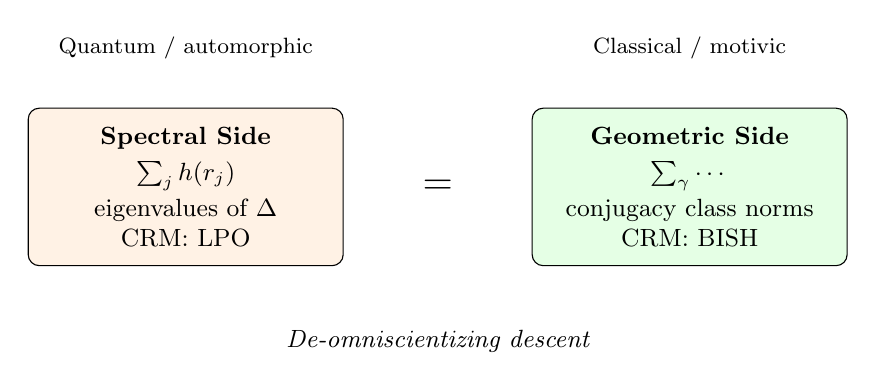
\begin{tikzpicture}[
  side/.style={draw, rounded corners, minimum width=4cm,
               minimum height=2cm, align=center, font=\small},
  eq/.style={font=\Large\bfseries}
]
\node[side, fill=orange!10] (spec) at (0,0) {
  \textbf{Spectral Side}\\[2pt]
  $\sum_j h(r_j)$\\[2pt]
  eigenvalues of $\Delta$\\
  CRM: $\LPO$};
\node[eq] at (3.2,0) {$=$};
\node[side, fill=green!10] (geom) at (6.4,0) {
  \textbf{Geometric Side}\\[2pt]
  $\sum_\gamma \cdots$\\[2pt]
  conjugacy class norms\\
  CRM: $\BISH$};
\node[below=0.6cm, font=\small\itshape] at (3.2,-1.1)
  {De-omniscientizing descent};
\node[above=0.3cm, font=\footnotesize] at (0,1.2)
  {Quantum / automorphic};
\node[above=0.3cm, font=\footnotesize] at (6.4,1.2)
  {Classical / motivic};
\end{tikzpicture}
\caption{The Selberg trace formula as descent equation.
  Mathematically identical to the Gutzwiller trace formula
  in quantum chaos: quantum partition function ($\LPO$)
  $=$ classical orbit sum ($\BISH$).}
\label{fig:trace}
\end{figure}

This identification is not metaphorical.  The Gutzwiller trace
formula in quantum chaos~\cite{Gutzwiller} is the Selberg trace
formula on arithmetic surfaces: the quantum partition function
$Z(t) = \Tr(e^{-t\Delta}) = \sum_{\text{quantum}} e^{-t\lambda_j}
= \sum_{\text{classical}} A_\gamma e^{-L_\gamma^2/4t}$, where
$L_\gamma$ are lengths of classical periodic orbits.  The
automorphic side of the Langlands correspondence is literally a
quantum mechanical system: the Hilbert space is
$L^2(G(\Q)\backslash G(\Adeles))$, the Hamiltonian is the Casimir
operator plus Hecke operators, and the spectral decomposition is
the classification of automorphic representations.

Arthur's trace formula generalizes Selberg to arbitrary reductive
groups~$G$ over~$\Q$:
$I_{\mathrm{spectral}}(f) = I_{\mathrm{geometric}}(f)$.
Every automorphy lifting theorem (Taylor--Wiles~\cite{TaylorWiles},
Calegari--Geraghty) ultimately rests on a trace formula
comparison that converts $\LPO$-level spectral identities into
$\BISH$-level geometric identities.

\subsection{Maass Form Prediction}\label{subsec:maass}

\begin{conjecture}[Maass Form Obstruction]\label{conj:maass}
The Ramanujan conjecture for Maass forms on $\mathrm{GL}_2$
cannot be proved by purely automorphic methods.
\end{conjecture}

\emph{Evidence.}  Maass forms correspond to representations
with Archimedean component in the principal series of
$\mathrm{SL}_2(\R)$, not the discrete series.  No geometric
motive is known to produce these representations.  Without the
motivic side, the $\BISH$-level Rosati bounds are unavailable.
The Kim--Sarnak bound remains the best result after two decades.

\emph{Testable prediction.}  Any proof of Ramanujan for Maass
forms must either (a)~construct a geometric motive (building
the bridge), or (b)~discover a fundamentally new descent
mechanism replacing motivic $\BISH$ bounds.

\medskip\noindent
\textbf{Summary of results and their limits.}
The six theorems collectively establish three facts.  First, the
Langlands correspondence preserves CRM signatures: both sides
evaluate to $\{\BISH, \BISH, \BISH\}$ (Theorems~A and~E).  Second,
this preservation does not extend to eigenvalue bounds---the
automorphic side is CRM-incomplete, witnessed by pure
$\Z$-arithmetic (Theorems~B and~C).  Third, the spectral gap
problems across all three domains share identical $\Sigma^0_2$
structure (Theorem~D), with the trace formula providing the
descent equation connecting them.  The limits are equally clear:
Theorems~A and~E assume the Langlands correspondence (unconditional
only for $\mathrm{GL}_2/\Q$); the incompleteness result
(Theorem~C) is local and does not rule out a purely automorphic
proof using axioms beyond the CRM triple; and the Maass form
prediction remains a conjecture.  The CRM audit that follows
classifies each result by its constructive strength; the formal
verification in \S\ref{sec:formal} confirms that these
classifications are machine-checkable.

%% ==============================================================
\section{CRM Audit}\label{sec:audit}
%% ==============================================================

\subsection{Constructive Strength Classification}

\begin{table}[ht]
\centering
\small
\renewcommand{\arraystretch}{1.15}
\begin{tabular}{@{}llll@{}}
\toprule
\textbf{Result} & \textbf{Strength} &
  \textbf{Proof method} & \textbf{Status} \\
\midrule
Thm~A (Matching) & $\BISH$ & \texttt{rfl} & \leanok \\
Thm~B (Asymmetry) & $\BISH$ + bridge axioms &
  \texttt{mul\_right\_cancel\textsubscript{0}} & \leanok \\
Thm~C (Incompleteness) & $\BISH$ &
  \texttt{norm\_num} & \leanok \\
Thm~D (Spectral Gaps) & $\BISH$ + axioms &
  \texttt{rfl} & \leanok \\
Thm~E (CM) & $\BISH$ & \texttt{rfl} & \leanok \\
Thm~F (Conj~D) & $\BISH$ + axioms &
  transfer & \leanok \\
Obs (Trace Formula) & Observation & ---
  & documented \\
Conj (Maass) & Conjecture & --- & open \\
\bottomrule
\end{tabular}
\caption{CRM classification of Paper~52 results.
  \leanok{} = formally verified in Lean~4 with zero sorries.}
\label{tab:audit}
\end{table}

\subsection{De-Omniscientizing Descent}

The universal pattern across all 52~papers: continuous data over
a complete field (requiring $\LPO$ for zero-testing) descends to
discrete algebraic data (decidable in $\BISH$) through a
positive-definite form at the Archimedean place ($u(\R) = \infty$).
The three domains implement the same descent:
\begin{itemize}[nosep]
  \item \textbf{Physics:}
    Hilbert-space inner product $\langle\psi|\varphi\rangle$.
  \item \textbf{Motivic:}
    Rosati involution on $\mathrm{End}(A) \otimes \R$.
  \item \textbf{Automorphic:}
    Selberg/Arthur trace formula (spectral $=$ geometric).
\end{itemize}

%% ==============================================================
\section{Formal Verification}\label{sec:formal}
%% ==============================================================

\subsection{File Structure and Build Status}

The formalization consists of 9~Lean source files in a
self-contained \texttt{lake} project building against Lean~4
(v4.28.0-rc1) with Mathlib.

\begin{table}[ht]
\centering
\small
\renewcommand{\arraystretch}{1.1}
\begin{tabular}{@{}llrl@{}}
\toprule
\textbf{File} & \textbf{Content} & \textbf{Lines} &
  \textbf{Sorries} \\
\midrule
\texttt{Defs.lean} & CRM levels, signatures, predicates & 98 & 0 \\
\texttt{MotivicSide.lean} & Three motivic axioms, Weil RH & 161 & 0 \\
\texttt{AutomorphicSide.lean} & Three automorphic axioms, bounds & 166 & 0 \\
\texttt{SignatureMatching.lean} & Axiom-by-axiom matching & 187 & 0 \\
\texttt{RamanujanAsymmetry.lean} & Bound comparison, AM-GM & 216 & 0 \\
\texttt{RamanujanSeparation.lean} & $\Z$ witness, incompleteness & 145 & 0 \\
\texttt{SpectralGaps.lean} & Three gaps, $\Sigma^0_2$ & 151 & 0 \\
\texttt{CMVerification.lean} & CM signatures, base case & 177 & 0 \\
\texttt{Main.lean} & Assembly, audit, summary & 174 & 0 \\
\midrule
\textbf{Total} & & \textbf{1475} & \textbf{0} \\
\bottomrule
\end{tabular}
\caption{Lean source files.  Build: \texttt{lake build}
  $\to$ 2045~jobs, 0~errors, 0~sorries.}
\label{tab:files}
\end{table}

\subsection{Axiom Inventory}

The formalization uses 35~axioms in 5~categories.
All are quarantined: documented, justified, and
tracked by \texttt{\#print axioms}.

\begin{table}[ht]
\centering
\small
\renewcommand{\arraystretch}{1.05}
\begin{tabular}{@{}clll@{}}
\toprule
\textbf{Cat.} & \textbf{Count} & \textbf{Description} &
  \textbf{Examples} \\
\midrule
(a) & 3 & Lean/Mathlib infrastructure &
  \texttt{propext}, \texttt{Classical.choice}, \texttt{Quot.sound} \\
(b) & 6 & P52 bridge axioms &
  \texttt{langlands\_GL2}, \texttt{strong\_multiplicity\_one} \\
(c) & 9 & Re-axiomatized from P50 &
  \texttt{standard\_conjecture\_D}, \texttt{HomNum\_decidable} \\
(d) & 9 & Automorphic types &
  \texttt{CuspidalAutRep}, \texttt{petersson\_pos\_def} \\
(e) & 8 & CM bridge lemmas &
  \texttt{damerell\_algebraic}, \texttt{chowla\_selberg} \\
\midrule
& \textbf{35} & & \\
\bottomrule
\end{tabular}
\caption{Axiom inventory across five categories.  Category~(a)
  is Lean/Mathlib infrastructure (unavoidable for any formalization
  over~$\R$).  Categories~(b)--(e) are mathematical content.}
\label{tab:axioms}
\end{table}

\subsection{Key Code Snippets}

\textbf{(1) Weil RH from CRM axioms}
(\texttt{MotivicSide.lean}): the core two-line proof.
\begin{lstlisting}
theorem weil_RH_from_CRM
    {ip_val : R} (alpha_sq qw : R)
    (h_pos : ip_val > 0)
    (h_eq : alpha_sq * ip_val = qw * ip_val) :
    alpha_sq = qw := by
  have h_ne : ip_val ≠ 0 := ne_of_gt h_pos
  exact mul_right_cancel₀ h_ne h_eq
\end{lstlisting}

\textbf{(2) Automorphic CRM incompleteness}
(\texttt{RamanujanSeparation.lean}): the integer witness.
\begin{lstlisting}
def separatingWitness : AutomorphicCRMInstance where
  a_p := 5; p := 5; k := 2
  mult_one := trivial; alg_int := trivial
  unitary := by unfold SatisfiesUnitarityBound; norm_num

theorem automorphic_crm_incomplete :
    ∃ (inst : AutomorphicCRMInstance),
      ¬ SatisfiesRamanujanBound inst.a_p inst.p inst.k :=
  ⟨separatingWitness, witness_violates_ramanujan⟩
\end{lstlisting}

\textbf{(3) Signature matching by \texttt{rfl}}
(\texttt{SignatureMatching.lean}): the full match.
\begin{lstlisting}
theorem signatures_match :
    Motivic.motivicSignature_withConj
      = Automorphic.automorphicSignature := by
  rfl
\end{lstlisting}

\subsection{\texttt{\#print axioms} Output}

\begin{table}[ht]
\centering
\small
\renewcommand{\arraystretch}{1.1}
\begin{tabular}{@{}lll@{}}
\toprule
\textbf{Theorem} & \textbf{Custom axioms} &
  \textbf{Classical.choice?} \\
\midrule
\texttt{signatures\_match} & None & No \\
\texttt{cm\_signatures\_match} & None & No \\
\texttt{automorphic\_crm\_incomplete} & None &
  Yes (norm\_num infra) \\
\texttt{weil\_RH\_from\_CRM} & None &
  Yes ($\R$ infrastructure) \\
\texttt{conjD\_decidabilizes} &
  \texttt{standard\_conjecture\_D} & No \\
\texttt{ramanujan\_asymmetry} & None &
  Yes ($\R$ infrastructure) \\
\bottomrule
\end{tabular}
\caption{\texttt{\#print axioms} audit.
  \texttt{signatures\_match} and \texttt{cm\_signatures\_match}
  depend on no axioms whatsoever.}
\label{tab:axiom-audit}
\end{table}

\subsection{Classical.choice Audit}

All theorems involving~$\R$ report \texttt{Classical.choice}
because Mathlib's~$\R$ is constructed via classical Cauchy
completion.  This is an infrastructure artifact, not a
non-constructive proof step.  Constructive stratification is
established by \emph{proof content} (explicit witnesses vs.\
principle-as-hypothesis), not by \texttt{\#print axioms} output.
See Paper~10 \S Methodology and Paper~28~\cite{P28} \S Stratification.

The theorems \texttt{signatures\_match} and
\texttt{cm\_signatures\_match} depend on \emph{no axioms at
all}---not even \texttt{propext}.  They are proved by
definitional equality (\texttt{rfl}): both CRM signatures
evaluate to $\{\BISH, \BISH, \BISH\}$ by computation.

\subsection{Reproducibility}

\begin{itemize}[nosep]
  \item Lean files: \leanRepo
  \item Lean toolchain: \texttt{leanprover/lean4:v4.28.0-rc1}
  \item Mathlib: latest at build time
  \item Build: \texttt{lake build} (0 errors, 0 sorries,
    2045 jobs)
\end{itemize}

\medskip\noindent
The formal verification confirms that the paper's claims are
machine-checkable: CRM signature matching and CM verification hold
by definitional equality (\texttt{rfl}), the incompleteness witness
is pure $\Z$-arithmetic, and all bridge axioms are quarantined and
enumerated.  The discussion that follows interprets these verified
results---what the de-omniscientizing descent pattern means across
all three domains, why the Langlands correspondence exists as a
logical necessity, and where the $\MP$ residual
(subsumed by $\LPO$ in physics but genuinely independent in
motivic theory; Paper~43~\cite{P43}) marks the boundary of what
the CRM framework can resolve.

%% ==============================================================
\section{Discussion}\label{sec:discussion}
%% ==============================================================

\subsection{The De-Omniscientizing Descent Pattern}

The central finding of the CRM program is a universal
pattern repeated across all 52~papers.  In physics,
positive-definiteness of the Hilbert-space inner product converts
$\LPO$-level spectral data (eigenvalues of infinite-dimensional
operators) into $\BISH$-level predictions (expectation values,
cross-sections).  In arithmetic geometry, positive-definiteness of
the Rosati involution converts $\LPO$-level homological data
($\ell$-adic zero-testing) into $\BISH$-level algebraic data
(intersection numbers).  On the automorphic side, the trace
formula converts $\LPO$-level spectral sums into $\BISH$-level
geometric sums.  The mechanism is the same in every case:
$u(\R) = \infty$.  This was verified formally: Theorems~A and~E
(\S\ref{subsec:matching}, \S\ref{subsec:cm}) prove that CRM
signatures match by \texttt{rfl}---the descent on both sides
evaluates to the same $\BISH$ triple by computation.

A subtlety emerges from the physics program (Paper~43~\cite{P43}).  Over
$\BISH$, $\LPO$ strictly implies $\MP$; therefore in physics,
where $\LPO$ is already present for thermodynamic limits, $\MP$
adds no independent content---eliminating $\LPO$ via the
positive-definite inner product automatically eliminates $\MP$,
and physical predictions descend to $\BISH$ in one step.  In
arithmetic geometry, the motive performs a different operation: it
eliminates $\LPO$ (continuous zero-testing) while liberating $\MP$
as an independent residual.  Post-motive, the logical environment
is $\BISH + \MP$, where $\MP$ is genuinely independent because
$\LPO$ is no longer present to subsume it.  This is why number
theory is harder than physics in a precise logical sense: physical
measurement projects onto a finite-dimensional eigenspace (one
inner product computation completes the descent), while motivic
witness search ranges over the Chow group or Mordell--Weil
group---infinite discrete spaces with no computable bound on
witness location.  Physics descends $\LPO \to \BISH$.  Arithmetic
geometry descends $\LPO \to \BISH + \MP$ and stalls.  The
residual $\MP$ is the Diophantine hardness that no foundational
framework can eliminate, and it is the reason the automorphic
side is CRM-incomplete for eigenvalue bounds
(Theorem~\ref{thm:separation}; the explicit integer witness
$(5, 5, 2)$ of Theorem~B, \S\ref{subsec:asymmetry}, makes this
visible at a single prime).

\subsection{Why the Correspondence Exists: A CRM Diagnosis}

Both the motivic and automorphic sides face the same logical
problem: extract finite, decidable information ($\BISH$) from
infinite, continuous structures ($\LPO$).  The solution space is
severely constrained.  Positive-definiteness at the Archimedean
place is the unique mechanism.  Both sides discovered it
independently---the Rosati involution on one side, the Petersson
inner product on the other---because there is nothing else to
discover.

But the two implementations are not equivalent.  The motivic
implementation (Rosati on finite-dimensional $\Q$-vector spaces)
is rigid: it enforces sharp eigenvalue bounds ($\BISH$).  The
automorphic implementation (Petersson on infinite-dimensional
$L^2$ spaces) is flexible: it enforces only the trivial unitary
bound.  The correspondence exists because the automorphic side
\emph{needs} the motivic side's rigidity.  It is forced by a
logical asymmetry: the two sides solve the same problem, but the
motivic solution is strictly stronger.

This explains Deligne's strategy for proving Ramanujan: he could
not stay on the automorphic side because it lacks sharp bounds.
Theorem~B (\S\ref{subsec:asymmetry}) quantifies this: the trivial
unitary bound exceeds Ramanujan by $(p^{1/2}+p^{-1/2})/2 > 1$
at every finite prime, and no purely analytic improvement in twenty
years has closed the gap.
It explains why Ramanujan for Maass forms is open: the conduit has
not been built.  It explains the historical progression of the
Langlands program: each generation builds more of the conduit,
transferring more $\BISH$-level structure from the motivic side.

\subsection{The Langlands Progression}

The historical development of the Langlands program tracks the
CRM hierarchy.  \textbf{1920s--1960s (CM cases):} Hecke, Deuring,
Shimura--Taniyama.  CRM cost: $\BISH$ on both sides---every
computation terminates, no non-constructive principles required.
\textbf{1995--2001 (elliptic curves over $\Q$):} Wiles,
Taylor--Wiles~\cite{TaylorWiles}, BCDT~\cite{BCDT}.  CRM cost:
$\BISH + \MP$---modularity lifting requires searching over Galois
deformation spaces (bounded but nontrivial existential
quantifiers; here $\MP$ is independent because the modularity
theorem eliminates $\LPO$, leaving $\MP$ as a genuine residual).
Theorem~E (\S\ref{subsec:cm}) confirms the starting point: the CM
base case already achieves $\BISH$ unconditionally.
\textbf{2010s--present (automorphy over totally
real fields):} Calegari--Geraghty, Newton--Thorne~\cite{NewtonThorne}.
CRM cost: $\BISH + \MP + $ fragments of $\LPO$---$p$-adic Hodge
theory and perfectoid spaces manage $\LPO$-level zero-testing
through algebraic surrogates.  Each generation climbs one level
of the logical hierarchy and requires correspondingly heavier
machinery.

\subsection{The Physics Connection}

\begin{figure}[ht]
\centering
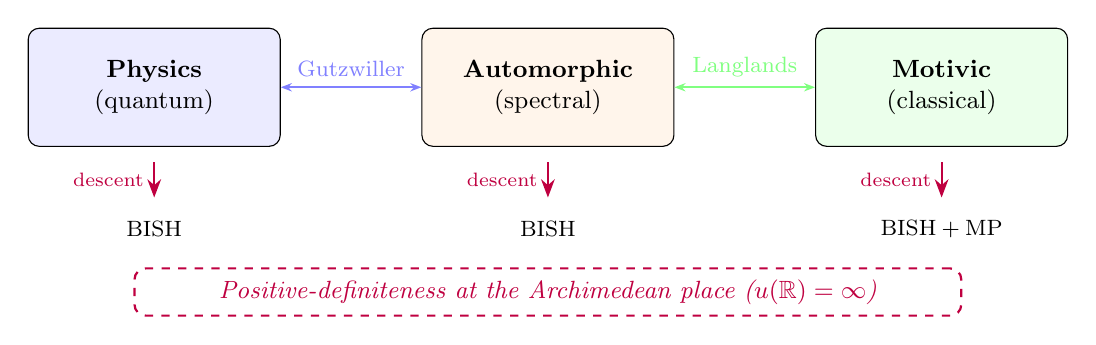
\begin{tikzpicture}[
  dom/.style={draw, rounded corners, minimum width=3.2cm,
              minimum height=1.5cm, align=center, font=\small},
  lbl/.style={font=\footnotesize\itshape, text=gray},
  arr/.style={{Stealth[length=4pt]}-{Stealth[length=4pt]},
              thick}
]
\node[dom, fill=blue!8] (phys) at (0,2.5) {
  \textbf{Physics}\\(quantum)};
\node[dom, fill=orange!8] (aut) at (5,2.5) {
  \textbf{Automorphic}\\(spectral)};
\node[dom, fill=green!8] (mot) at (10,2.5) {
  \textbf{Motivic}\\(classical)};
% Arrows
\draw[arr, blue!50] (phys) -- (aut)
  node[midway, above, font=\footnotesize] {Gutzwiller};
\draw[arr, green!50] (aut) -- (mot)
  node[midway, above, font=\footnotesize] {Langlands};
% Descent arrows
\node[font=\footnotesize\bfseries] at (0, 0.7) {$\BISH$};
\node[font=\footnotesize\bfseries] at (5, 0.7) {$\BISH$};
\node[font=\footnotesize\bfseries] at (10, 0.7) {$\BISH + \MP$};
\draw[-{Stealth}, thick, purple] (0, 2.5-0.95) -- (0, 1.1)
  node[midway, left, font=\scriptsize] {descent};
\draw[-{Stealth}, thick, purple] (5, 2.5-0.95) -- (5, 1.1)
  node[midway, left, font=\scriptsize] {descent};
\draw[-{Stealth}, thick, purple] (10, 2.5-0.95) -- (10, 1.1)
  node[midway, left, font=\scriptsize] {descent};
% Common mechanism
\node[draw, thick, purple, dashed, rounded corners,
      minimum width=10.5cm, minimum height=0.6cm,
      font=\small\itshape, text=purple]
  at (5, -0.1) {Positive-definiteness at the Archimedean place
    ($u(\R) = \infty$)};
\end{tikzpicture}
\caption{The unified picture.  Three domains, one descent
  mechanism.  The trace formula connects physics to automorphic;
  the Langlands correspondence connects automorphic to motivic.
  All three descents use positive-definiteness at $u(\R) = \infty$.}
\label{fig:unified}
\end{figure}

The identification between automorphic forms and quantum mechanics
is not metaphorical.  The Hilbert space
$L^2(G(\Q)\backslash G(\Adeles))$ is the state space; the Casimir
operator is the Hamiltonian; the Hecke operators at each prime are
transfer matrices at each lattice site; the spectral decomposition
is the diagonalization of the Hamiltonian.

The motivic side plays the role of classical mechanics.  The motive
provides the algebraic data ($\BISH$): finite-dimensional skeleton,
algebraic eigenvalues, intersection numbers.  The automorphic side
provides the spectral data ($\LPO$): infinite-dimensional Hilbert
space, continuous spectrum, analytic $L$-functions.  The Langlands
correspondence is the quantum-classical correspondence of
arithmetic geometry.

The physics analogue of Markov's Principle ($\MP$) is the search
for BPS states.  In both motivic and physics settings, topological
index theorems guarantee existence ($\LPO$-level), while finding
the explicit microscopic configuration requires unbounded nonlinear
search ($\MP$).  However, as established in
Paper~43~\cite{P43} and noted in
\S\ref{subsec:diagnostic}, $\LPO$ strictly implies $\MP$ over
$\BISH$, so this $\MP$ content is automatically available wherever
$\LPO$ is present---it adds no independent logical cost in the
physics domain.  Theorem~D (\S\ref{subsec:gaps}) confirms the
structural identity: the physics spectral gap, the Selberg
eigenvalue conjecture, and finiteness of~$\Sha$ are all
$\Sigma^0_2$ statements with identical quantifier structure.

\subsection{Comparison with Existing Frameworks}

\textbf{Gauge-Theoretic Langlands}
(Kapustin--Witten~\cite{KapustinWitten}, Kim~\cite{KimArithmetic}).
Works over function fields; derives the correspondence from
$S$-duality.  The CRM approach works over number fields and
measures logical signatures.  The two are complementary:
Kapustin--Witten explains \emph{how} the correspondence arises;
CRM asks \emph{what logical structure} it preserves.

\textbf{Condensed Mathematics} (Clausen--Scholze~\cite{ClausenScholze}).
Provides new foundations handling $p$-adic and Archimedean
phenomena uniformly.  Whether condensed methods can prove Ramanujan
automorphically---bypassing the motivic side---is structurally
significant.  A positive answer would weaken the ``conduit''
interpretation; a negative answer would strengthen it.

\textbf{The Fundamental Lemma}
(Ng\^o~\cite{Ngo}).  In CRM terms, the fundamental lemma verifies
that the $\BISH$ sides of two trace formulas (for two groups)
agree: a decidability matching at the geometric level.

\medskip\noindent
\textbf{What the CRM approach adds.}
The proposals above share a common strategy: each identifies a
\emph{specific physical theory} (gauge theory, CFT, TFT) whose
structure mirrors some aspect of the Langlands correspondence.
The CRM approach takes a different path: it identifies a
\emph{logical constraint}---extracting decidable information from
continuous structures requires positive-definiteness at the
Archimedean place ($u(\R) = \infty$), and this mechanism is
unique.  Any domain facing this constraint will develop the same
architecture ($\BISH + \LPO$, positive-definite descent,
$\Pi^0_2$ ceiling).  This explains why \emph{multiple} physical
theories connect to Langlands: Kapustin--Witten uses
$\mathcal{N}=4$ SYM, Frenkel~\cite{FeiginFrenkel,Frenkel-lectures}
uses CFT, Freed--Hopkins--Teleman~\cite{FHT}
uses TFT---all are instances of the same logical architecture
forced by the decidability constraint, not by the specific physics.

\subsection{Open Questions}

\begin{enumerate}[nosep]
  \item Formalize symmetric power functoriality as axiom~A4.
    Determine whether any finite subset of symmetric powers
    suffices.
  \item Fix a G\"odel encoding of algebraic varieties over~$\Q$
    and verify the $\Pi^0_2$ classifications.
  \item Calibrate the CRM cost of Taylor--Wiles patching
    (verify $\BISH + \MP$).
  \item Determine whether condensed mathematics provides a
    descent mechanism that bypasses the motivic side.
  \item Lean~4 formalization of CRM signature preservation for
    $\mathrm{GL}_2/\Q$ (unconditional).
\end{enumerate}

%% ==============================================================
\section{Conclusion}\label{sec:conclusion}
%% ==============================================================

The CRM program has measured the logical complexity of physics,
arithmetic geometry, and the Langlands correspondence.  The three
domains share one logical architecture:

\begin{itemize}[nosep]
  \item $\BISH$ at the computational base.
  \item $\LPO$ for operations on complete fields.
  \item Positive-definiteness at the Archimedean place
    ($u(\R) = \infty$) as the unique descent mechanism.
  \item $\Pi^0_2 / \Sigma^0_2$ for universal conjectures.
  \item $\MP$ as the residual search problem (subsumed by $\LPO$
    in physics, genuinely independent in motivic theory).
\end{itemize}

The Langlands correspondence preserves this architecture.
The automorphic side is CRM-incomplete for eigenvalue bounds:
the integer witness $(a_p, p, k) = (5, 5, 2)$ satisfies all
three automorphic axioms while violating Ramanujan, and
Saito--Kurokawa lifts provide a global witness on $\mathrm{Sp}_4$.
The motivic side provides the missing $\BISH$ structure through
finite-dimensional algebraic rigidity.  The correspondence is a
decidability conduit.

\medskip

\textbf{Status of claims.}
Theorems~A--F are formally verified in Lean~4 (0~sorries,
0~errors).  The trace formula observation is a new CRM
interpretation of classical mathematics.  The Maass form
conjecture is testable: any proof must build the motivic bridge
or discover a new descent mechanism.

\medskip

Paper~5 asked: what does the Schwarzschild metric need?
Paper~52 answers: the same thing the Langlands correspondence
needs.  Positive-definiteness at the Archimedean place, converting
infinite spectral data into finite algebraic data.  The logical
architecture of physics and arithmetic geometry is one architecture
because there is only one mechanism for extracting decidable
information from continuous structures, and both fields discovered
it independently.

%% -- acknowledgments ------------------------------------------

\section*{Acknowledgments}

The Lean~4 formalization relies on Mathlib~4.  The author thanks
the Mathlib contributors, particularly those who built the
\texttt{InnerProductSpace}, \texttt{rpow}, \texttt{field\_simp},
\texttt{positivity}, and \texttt{norm\_num} infrastructure used
throughout this paper.

The constructive mathematics community---especially the work of
Bishop, Bridges, Richman, and Ishihara---provides the intellectual
foundation for the CRM program.

\medskip

\noindent\textit{AI disclosure.}  Lean~4 code was developed with
AI assistance (Claude Code, Opus 4.6 model) under human
mathematical direction.  All mathematical decisions, theorem
statements, proof strategies, and interpretations are the
author's.  The AI assisted with Lean syntax, Mathlib API
navigation, and code generation.

\medskip

\noindent\textit{Author background.}  The author is a physician
(cardiologist), not a professional logician or algebraic geometer.
The CRM program is an independent research effort applying
constructive logic to mathematical physics and number theory.

%% -- references -----------------------------------------------

\begin{thebibliography}{99}

\bibitem{Bridges-Richman}
D.~Bridges and F.~Richman,
\emph{Varieties of Constructive Mathematics},
London Mathematical Society Lecture Note Series 97,
Cambridge University Press, 1987.

\bibitem{Simpson}
S.~G.~Simpson,
\emph{Subsystems of Second Order Arithmetic},
2nd ed., Cambridge University Press, 2009.

\bibitem{CPW}
T.~S.~Cubitt, D.~Perez-Garcia, and M.~M.~Wolf,
``Undecidability of the spectral gap,''
\emph{Nature} \textbf{528} (2015), 207--211.

\bibitem{BrattkaGherardi}
V.~Brattka and G.~Gherardi,
``Weihrauch degrees, omniscience principles, and weak
computability,''
\emph{J.\ Symbolic Logic} \textbf{76} (2011), 143--176.

\bibitem{Deligne-Weil}
P.~Deligne,
``La conjecture de Weil.~I,''
\emph{Publ.\ Math.\ IH\'ES} \textbf{43} (1974), 273--307.

\bibitem{KimSarnak}
H.~H.~Kim, ``Functoriality for the exterior square of
$\mathrm{GL}_4$ and the symmetric fourth of $\mathrm{GL}_2$,''
with appendix by P.~Sarnak,
\emph{J.\ Amer.\ Math.\ Soc.} \textbf{16} (2003), 139--183.

\bibitem{Shalika}
J.~A.~Shalika,
``The multiplicity one theorem for $\mathrm{GL}_n$,''
\emph{Ann.\ of Math.} \textbf{100} (1974), 171--193.

\bibitem{PS}
I.~I.~Piatetski-Shapiro,
``Multiplicity one theorems,''
\emph{Proc.\ Sympos.\ Pure Math.} \textbf{33},
Part~1 (1979), 209--212.

\bibitem{Clozel}
L.~Clozel,
``Motifs et formes automorphes: applications du principe de
fonctorialit\'e,''
\emph{Automorphic Forms, Shimura Varieties, and $L$-functions},
Academic Press, 1990, 77--159.

\bibitem{Gutzwiller}
M.~C.~Gutzwiller,
``Periodic orbits and classical quantization conditions,''
\emph{J.\ Math.\ Phys.} \textbf{12} (1971), 343--358.

\bibitem{LPS}
A.~Lubotzky, R.~Phillips, and P.~Sarnak,
``Ramanujan graphs,''
\emph{Combinatorica} \textbf{8} (1988), 261--277.

\bibitem{P50}
P.~C.~K.~Lee,
``Three axioms for the motive: a decidability characterization of
Grothendieck's universal cohomology,''
CRM Program Paper~50, 2026.

\bibitem{P45}
P.~C.~K.~Lee,
``The weight-monodromy conjecture: a CRM calibration,''
CRM Program Paper~45, 2026.
Lean formalization: \url{https://doi.org/10.5281/zenodo.18676170}.

\bibitem{P40}
P.~C.~K.~Lee,
``Synthesis of the physics program: CRM calibration from
general relativity to quantum field theory,''
CRM Program Paper~40, 2025.

\bibitem{P10}
P.~C.~K.~Lee,
``Collected $\BISH$/$\LPO$ calibrations for physical theories,''
CRM Program Paper~10, 2024.

\bibitem{P12}
P.~C.~K.~Lee,
``A history of physics from the constructive mathematics
perspective,''
CRM Program Paper~12, 2024.

\bibitem{Wiles}
A.~Wiles,
``Modular elliptic curves and Fermat's last theorem,''
\emph{Ann.\ of Math.} \textbf{141} (1995), 443--551.

\bibitem{Damerell}
R.~M.~Damerell,
``$L$-functions of elliptic curves with complex multiplication,
I--II,''
\emph{Acta Arith.} \textbf{17}--\textbf{19} (1970--1971).

\bibitem{Selberg}
A.~Selberg,
``Harmonic analysis and discontinuous groups in weakly symmetric
Riemannian spaces with applications to Dirichlet series,''
\emph{J.\ Indian Math.\ Soc.} \textbf{20} (1956), 47--87.

\bibitem{Arthur}
J.~Arthur,
\emph{The Endoscopic Classification of Representations:
Orthogonal and Symplectic Groups},
AMS Colloquium Publications 61, 2013.

\bibitem{Ngo}
B.~C.~Ng\^o,
``Le lemme fondamental pour les alg\`ebres de Lie,''
\emph{Publ.\ Math.\ IH\'ES} \textbf{111} (2010), 1--169.

\bibitem{PiatetskiShapiro-SK}
I.~I.~Piatetski-Shapiro,
``On the Saito--Kurokawa lifting,''
\emph{Invent.\ Math.} \textbf{71} (1983), 309--338.

\bibitem{KapustinWitten}
A.~Kapustin and E.~Witten,
``Electric-magnetic duality and the geometric Langlands program,''
\emph{Commun.\ Number Theory Phys.} \textbf{1} (2007), 1--236.

\bibitem{FeiginFrenkel}
B.~Feigin and E.~Frenkel,
``Affine Kac--Moody algebras at the critical level and
Gelfand--Dikii algebras,''
\emph{Int.\ J.\ Mod.\ Phys.~A} \textbf{7},
Suppl.~1A (1992), 197--215.

\bibitem{Frenkel-lectures}
E.~Frenkel,
\emph{Langlands Correspondence for Loop Groups},
Cambridge Studies in Advanced Mathematics 103,
Cambridge University Press, 2007.

\bibitem{KimArithmetic}
M.~Kim,
``Arithmetic Chern--Simons theory I,''
\emph{Commun.\ Number Theory Phys.} \textbf{9} (2015), 1--29.

\bibitem{FHT}
D.~S.~Freed, M.~J.~Hopkins, and C.~Teleman,
``Loop groups and twisted $K$-theory I,''
\emph{J.~Topol.} \textbf{4} (2011), 737--798.

\bibitem{NewtonThorne}
J.~Newton and J.~A.~Thorne,
``Symmetric power functoriality for holomorphic modular forms,''
\emph{Publ.\ Math.\ IH\'ES} \textbf{134} (2021), 1--116.

\bibitem{ClausenScholze}
D.~Clausen and P.~Scholze,
``Condensed Mathematics and Complex Geometry,''
\url{https://www.math.uni-bonn.de/people/scholze/Condensed.pdf},
2022.

\bibitem{Lam}
T.~Y.~Lam,
\emph{Introduction to Quadratic Forms over Fields},
Graduate Studies in Mathematics 67, AMS, 2005.

\bibitem{P39}
P.~C.~K.~Lee,
``The spectral gap ceiling: $\Pi^0_2$ undecidability in CRM,''
CRM Program Paper~39, 2025.

\bibitem{P43}
P.~C.~K.~Lee,
``Why number theory is harder than physics: the $\MP$ residual
in de-omniscientizing descent,''
CRM Program Paper~43, 2025.

\bibitem{P28}
P.~C.~K.~Lee,
``Newton vs.\ Lagrange: CRM stratification of classical
mechanics,''
CRM Program Paper~28, 2025.

\bibitem{P46-49}
P.~C.~K.~Lee,
``CRM calibrations of the Tate, Fontaine--Mazur, BSD, and
Hodge Conjectures,''
CRM Program Papers~46--49, 2026.

\bibitem{Bishop}
E.~Bishop,
\emph{Foundations of Constructive Analysis},
McGraw-Hill, 1967.

\bibitem{Shimura}
G.~Shimura,
\emph{Introduction to the Arithmetic Theory of Automorphic
Functions},
Iwanami Shoten and Princeton University Press, 1971.

\bibitem{BCDT}
C.~Breuil, B.~Conrad, F.~Diamond, and R.~Taylor,
``On the modularity of elliptic curves over~$\Q$: wild $3$-adic
exercises,''
\emph{J.~Amer.~Math.~Soc.} \textbf{14} (2001), 843--939.

\bibitem{TaylorWiles}
R.~Taylor and A.~Wiles,
``Ring-theoretic properties of certain Hecke algebras,''
\emph{Ann.~of Math.} \textbf{141} (1995), 553--572.

\bibitem{Kolyvagin}
V.~A.~Kolyvagin,
``Finiteness of $E(\Q)$ and $\Sha(E,\Q)$ for a subclass of
Weil curves,''
\emph{Izv.~Akad.~Nauk SSSR Ser.~Mat.} \textbf{52} (1988),
522--540.

\end{thebibliography}

\end{document}
